%% ═══════════════════════════════════════════════════════════════════════════
%%  B.Tech Final Year Project Thesis
%%  Birsa Institute of Technology (BIT), Sindri
%%  Department of Civil Engineering
%%  Academic Year 2025–2026
%% ═══════════════════════════════════════════════════════════════════════════
\documentclass[12pt,a4paper,oneside]{report}

%% ─── Packages ────────────────────────────────────────────────────────────
\usepackage[T1]{fontenc}
\usepackage[utf8]{inputenc}
\usepackage{lmodern}
\usepackage{microtype}
\usepackage[a4paper,top=1in,bottom=1in,left=1.5in,right=1in]{geometry}
\usepackage{setspace}\onehalfspacing
\usepackage{amsmath,amssymb}
\usepackage{graphicx}
\graphicspath{{figures/}{../figures/}}
\usepackage{booktabs,tabularx,multirow,longtable}
\usepackage[table]{xcolor}
\definecolor{rowgray}{RGB}{245,245,248}
\usepackage{caption,subcaption}
\usepackage{float}
\usepackage[numbers,sort&compress]{natbib}
\usepackage{url}
\emergencystretch=1em
\usepackage{hyperref}
\hypersetup{colorlinks=true,linkcolor=blue!60!black,citecolor=blue!60!black,urlcolor=blue!60!black}
\usepackage[capitalise,noabbrev]{cleveref}
\usepackage{fancyhdr}
\usepackage{titlesec}
% \usepackage{tocloft}  % removed — not used, speeds compile
\usepackage{appendix}
\usepackage{enumitem}
% \usepackage{siunitx}  % removed — replaced \SI{} with manual formatting for portability
%% listings/algorithm packages removed (unused) to speed Overleaf compile

%% ─── Header / Footer ────────────────────────────────────────────────────
\pagestyle{fancy}
\fancyhf{}
\fancyhead[R]{\small\thepage}
\fancyhead[L]{\small\leftmark}
\renewcommand{\headrulewidth}{0.4pt}

%% ─── Chapter titles ─────────────────────────────────────────────────────
\titleformat{\chapter}[display]
  {\normalfont\Large\bfseries}
  {\chaptertitlename\ \thechapter}{16pt}{\LARGE}
\titlespacing*{\chapter}{0pt}{-20pt}{30pt}

%% ─── Custom commands ────────────────────────────────────────────────────
\newcommand{\dS}{\Delta S}
\newcommand{\dSobs}{\Delta S_{\mathrm{obs}}}
\newcommand{\dSclim}{\Delta S_{\mathrm{climate}}}
\newcommand{\dSanthro}{\Delta S_{\mathrm{anthro}}}
\newcommand{\BCM}{\,\mathrm{BCM}}
\newcommand{\NSE}{\mathrm{NSE}}
\newcommand{\KGE}{\mathrm{KGE}}

%% ═══════════════════════════════════════════════════════════════════════════
\begin{document}

%% ─── TITLE PAGE ──────────────────────────────────────────────────────────
\begin{titlepage}
\newgeometry{top=1in,bottom=1in,left=1in,right=1in}
\begin{center}

\vfill

{\fontfamily{phv}\selectfont\fontsize{16}{20}\bfseries
SATELLITE-BASED ATTRIBUTION OF\\[3pt]
ANTHROPOGENIC STORAGE SIGNALS IN\\[3pt]
DAMODAR VALLEY CORPORATION RESERVOIRS\\[3pt]
USING EXPLAINABLE MACHINE LEARNING\\[3pt]
AND CAUSAL INFERENCE}

\vspace{0.6cm}


\includegraphics[height=1in]{jut_logo}

\vspace{0.4cm}

{\fontfamily{ptm}\selectfont\fontsize{14}{17}\bfseries\itshape
A Project Report}\\[3pt]
{\fontfamily{ptm}\selectfont\fontsize{12}{15}\itshape
Submitted to}\\[3pt]
{\fontfamily{phv}\selectfont\fontsize{13}{16}\bfseries
JHARKHAND UNIVERSITY OF TECHNOLOGY, RANCHI}\\[3pt]
{\fontfamily{ptm}\selectfont\fontsize{11}{14}\itshape
In Partial Fulfillment of the Requirement for the Award of Degree of}

\vspace{0.4cm}

{\fontfamily{phv}\selectfont\fontsize{15}{18}\bfseries
BACHELOR OF TECHNOLOGY IN\\[3pt]
CIVIL ENGINEERING}

\vspace{0.4cm}

{\fontfamily{ptm}\selectfont\fontsize{12}{15}\selectfont Submitted by}\\[4pt]
{\fontfamily{phv}\selectfont\fontsize{14}{17}\bfseries
Nishi Kant Mandal\quad(22030430063)}

\vspace{0.4cm}

{\fontfamily{ptm}\selectfont\fontsize{12}{15}\selectfont Under the guidance of}\\[4pt]
{\fontfamily{phv}\selectfont\fontsize{14}{17}\bfseries
Dr.\ Maya Rajnarayan Ray}\\[3pt]
{\fontfamily{phv}\selectfont\fontsize{11}{14}\selectfont
Associate Professor}

\vspace{0.4cm}


\includegraphics[height=1in]{bit_sindri_logo}

\vspace{0.3cm}

{\fontfamily{phv}\selectfont\fontsize{13}{16}\bfseries
DEPARTMENT OF CIVIL ENGINEERING,}\\[3pt]
{\fontfamily{phv}\selectfont\fontsize{13}{16}\bfseries
BIT SINDRI,}\\[3pt]
{\fontfamily{phv}\selectfont\fontsize{13}{16}\bfseries
DHANBAD--828123 (JHARKHAND)}

\vspace{0.3cm}

{\fontfamily{phv}\selectfont\fontsize{14}{17}\bfseries June 2026}

\vfill

\end{center}
\restoregeometry
\end{titlepage}

%% ─── INSIDE COVER PAGE (identical to cover) ─────────────────────────────
\begin{titlepage}
\newgeometry{top=1in,bottom=1in,left=1in,right=1in}
\begin{center}

\vfill

{\fontfamily{phv}\selectfont\fontsize{16}{20}\bfseries
SATELLITE-BASED ATTRIBUTION OF\\[3pt]
ANTHROPOGENIC STORAGE SIGNALS IN\\[3pt]
DAMODAR VALLEY CORPORATION RESERVOIRS\\[3pt]
USING EXPLAINABLE MACHINE LEARNING\\[3pt]
AND CAUSAL INFERENCE}

\vspace{0.6cm}


\includegraphics[height=1in]{jut_logo}

\vspace{0.4cm}

{\fontfamily{ptm}\selectfont\fontsize{14}{17}\bfseries\itshape
A Project Report}\\[3pt]
{\fontfamily{ptm}\selectfont\fontsize{12}{15}\itshape
Submitted to}\\[3pt]
{\fontfamily{phv}\selectfont\fontsize{13}{16}\bfseries
JHARKHAND UNIVERSITY OF TECHNOLOGY, RANCHI}\\[3pt]
{\fontfamily{ptm}\selectfont\fontsize{11}{14}\itshape
In Partial Fulfillment of the Requirement for the Award of Degree of}

\vspace{0.4cm}

{\fontfamily{phv}\selectfont\fontsize{15}{18}\bfseries
BACHELOR OF TECHNOLOGY IN\\[3pt]
CIVIL ENGINEERING}

\vspace{0.4cm}

{\fontfamily{ptm}\selectfont\fontsize{12}{15}\selectfont Submitted by}\\[4pt]
{\fontfamily{phv}\selectfont\fontsize{14}{17}\bfseries
Nishi Kant Mandal\quad(22030430063)}

\vspace{0.4cm}

{\fontfamily{ptm}\selectfont\fontsize{12}{15}\selectfont Under the guidance of}\\[4pt]
{\fontfamily{phv}\selectfont\fontsize{14}{17}\bfseries
Dr.\ Maya Rajnarayan Ray}\\[3pt]
{\fontfamily{phv}\selectfont\fontsize{11}{14}\selectfont
Associate Professor}

\vspace{0.4cm}


\includegraphics[height=1in]{bit_sindri_logo}

\vspace{0.3cm}

{\fontfamily{phv}\selectfont\fontsize{13}{16}\bfseries
DEPARTMENT OF CIVIL ENGINEERING,}\\[3pt]
{\fontfamily{phv}\selectfont\fontsize{13}{16}\bfseries
BIT SINDRI,}\\[3pt]
{\fontfamily{phv}\selectfont\fontsize{13}{16}\bfseries
DHANBAD--828123 (JHARKHAND)}

\vspace{0.3cm}

{\fontfamily{phv}\selectfont\fontsize{14}{17}\bfseries June 2026}

\vfill

\end{center}
\restoregeometry
\end{titlepage}

%% ─── DECLARATION CERTIFICATE (from Supervisor) ──────────────────────────
\newpage
\thispagestyle{empty}

\vspace*{0.5cm}

\begin{center}
{\large\bfseries JHARKHAND UNIVERSITY OF TECHNOLOGY, JHARKHAND}\\[12pt]
{\normalsize\bfseries\underline{CERTIFICATE OF DECLARATION FROM THE SUPERVISOR}}
\end{center}

\vspace{1cm}

\noindent This is to certify that the work presented in the dissertation entitled
\textbf{``Satellite-Based Attribution of Anthropogenic Storage Signals in
Damodar Valley Corporation Reservoirs Using Explainable Machine Learning and
Causal Inference''} in partial fulfillment of the requirement for the award
of Degree of \textbf{Bachelor of Technology} in \textbf{Civil Engineering}
at \textbf{BIT Sindri} is an authentic work carried out under my supervision
and guidance.

\vspace{0.8cm}

\noindent To the best of my knowledge, the content of this thesis does not
form a basis for the award of any previous Degree to anyone else.

\vspace{2.5cm}

\noindent\begin{tabular}{p{0.45\textwidth}p{0.45\textwidth}}
  \textbf{Date:} \rule{3cm}{0.4pt} & \vspace{1.8cm} \\[1.8cm]
  & \rule{6cm}{0.4pt} \\[3pt]
  & \textbf{Dr.\ Maya Rajnarayan Ray} \\
  & Associate Professor \\
  & Dept.\ of Civil Engineering \\
  & BIT Sindri, Dhanbad \\
\end{tabular}


%% ─── CERTIFICATE OF APPROVAL (from Examiners) ──────────────────────────
\newpage
\thispagestyle{empty}

\vspace*{0.5cm}

\begin{center}
{\large\bfseries JHARKHAND UNIVERSITY OF TECHNOLOGY, JHARKHAND}\\[12pt]
{\normalsize\bfseries\underline{CERTIFICATE OF APPROVAL FROM THE EXAMINERS}}
\end{center}

\vspace{1cm}

\noindent The foregoing dissertation entitled \textbf{``Satellite-Based
Attribution of Anthropogenic Storage Signals in Damodar Valley Corporation
Reservoirs Using Explainable Machine Learning and Causal Inference''}, is
hereby approved as a creditable study of research topic and has been presented
in satisfactory manner to warrant its acceptance as prerequisite to the degree
for which it has been submitted.

\vspace{0.8cm}

\noindent It is understood that by this approval, the undersigned do not
necessarily endorse any conclusion drawn or opinion expressed therein, but
approve the thesis for the purpose for which it is submitted.

\vspace{3cm}

\noindent\begin{tabular}{p{0.45\textwidth}p{0.45\textwidth}}
  & \\
  \rule{5cm}{0.4pt} & \rule{5cm}{0.4pt} \\
  \textbf{(Internal Examiner)} & \textbf{(External Examiner)} \\
\end{tabular}

\vspace{3cm}

\begin{center}
\rule{5cm}{0.4pt}\\
\textbf{(Chairman)}\\[1cm]
\textbf{Head of the Department}
\end{center}

%% ─── DECLARATION (by Student) ───────────────────────────────────────────
\newpage
\thispagestyle{empty}
\begin{center}
{\Large\bfseries DECLARATION}
\end{center}

\vspace{1cm}

\noindent I hereby declare that the project work entitled
\textbf{``Satellite-Based Attribution of Anthropogenic Storage Signals in
Damodar Valley Corporation Reservoirs Using Explainable Machine Learning and
Causal Inference''} is an authentic record of my own work carried out during
the academic year 2025--2026 as a requirement for the award of the degree of
Bachelor of Technology in Civil Engineering from BIT Sindri, Dhanbad.

\vspace{0.5cm}

\noindent The work presented in this thesis has not been submitted to any
other university or institute for the award of any degree or diploma.

\vspace{0.5cm}

\noindent All sources of information have been duly acknowledged.

\vspace{2cm}

\noindent\begin{tabular}{l}
  \textbf{Nishi Kant Mandal} \\
  Registration No.\ 22030430063 \\
  B.Tech Civil Engineering \\
  BIT Sindri, Dhanbad \\[1cm]
  Date: \rule{3cm}{0.4pt}
\end{tabular}

%% ─── ACKNOWLEDGEMENTS ───────────────────────────────────────────────────
\newpage
\thispagestyle{empty}
\begin{center}
{\Large\bfseries ACKNOWLEDGEMENTS}
\end{center}

\vspace{1cm}

\noindent
I owe a great deal to my project supervisor, \textbf{Dr.\ Maya Rajnarayan
Ray}, Associate Professor in the Department of Civil Engineering at BIT
Sindri, for her steady guidance, encouragement, and patience throughout this
work. She gave me the freedom to explore an unconventional approach
--- satellite remote sensing combined with machine learning for a problem
usually tackled with in-situ data --- and that freedom gave me the
confidence to try something ambitious.

I am grateful to the \textbf{Head of the Department of Civil Engineering}
and the faculty of BIT Sindri for the academic environment and resources
that made this project possible. I also thank the \textbf{Central Water
Commission} (Ministry of Jal Shakti, Government of India) for making
reservoir storage bulletins publicly available, and the \textbf{Google Earth
Engine} team for providing free computational infrastructure for satellite
data processing.

This project relied entirely on open-source data and open-source tools. I
thank the developers of Python, XGBoost, SHAP, pyEDM, statsmodels, and the
many other libraries that made the analysis possible without any financial
expenditure. Working under that constraint was difficult at times, but in
hindsight it taught me a lot about resourcefulness.

Finally, I thank my family for their support, and my friends at BIT Sindri
who put up with my late-night debugging sessions and my growing obsession
with reservoir water levels. Whatever merit this work has belongs partly to
all of them; the errors are entirely my own.

\vspace{1cm}

\hfill\textbf{Nishi Kant Mandal}\\
\hfill Sindri, June 2026

%% ─── ABSTRACT ────────────────────────────────────────────────────────────
\newpage
\thispagestyle{empty}
\begin{center}
{\Large\bfseries ABSTRACT}
\end{center}

\vspace{0.5cm}

\noindent
Reservoir operations are a dominant but poorly understood source of
terrestrial water storage variability in managed river basins. Satellite
missions like the Gravity Recovery and Climate Experiment Follow-On
(GRACE-FO) measure total water storage changes at basin scale, yet they
cannot distinguish between climate-driven processes and deliberate human
management decisions at individual reservoirs. This matters because water
policy in India increasingly relies on GRACE-derived estimates of groundwater
depletion and water stress. In basins where reservoir operations contribute
substantially to the observed storage signal, these estimates may be
systematically biased.

We developed a six-stage satellite-based framework to isolate and characterise
anthropogenic storage signals in the Damodar Valley Corporation (DVC)
reservoir cascade in Jharkhand and West Bengal, using Sentinel-1 C-band
Synthetic Aperture Radar (SAR) imagery, GRACE-FO mascon data, and climate
reanalysis products. We reconstructed monthly storage anomalies for Maithon
Dam and Durgapur Barrage over 2017--2024 and validated them against nine
independent measurements from the Central Water Commission (CWC; RMSE =
0.07\,m, $n = 8$). An eXtreme Gradient Boosting (XGBoost) model trained on
eight climate drivers achieved modest predictive skill (Nash-Sutcliffe
Efficiency, $\NSE = 0.208$ on unclipped rows). Climate alone explains very
little of month-to-month storage variability in a managed reservoir. The
anthropogenic residual ranged from $-0.19$ to $+0.23$ Billion Cubic Metres
(BCM). Convergent Cross-Mapping (CCM) with 999 phase-randomised surrogates
confirmed that this residual is causally independent of all climate
predictors. Partial regression against GRACE-FO showed that the anthropogenic
signal remains detectable even after removing shared monsoon seasonality
($p = 0.0003$). A Dynamic Time Warping (DTW) based operational fingerprint
taxonomy (silhouette = 0.49) showed that DVC operational patterns can be
learned from satellite data alone, without any in-situ sensors.

\textbf{Keywords:} reservoir operations, Damodar Valley Corporation,
Sentinel-1 SAR, GRACE-FO, XGBoost, SHapley Additive exPlanations,
convergent cross-mapping, operational fingerprint taxonomy

%% ─── TABLE OF CONTENTS ──────────────────────────────────────────────────
\newpage
\tableofcontents
\newpage
\listoffigures
\newpage
\listoftables

%% ─── ABBREVIATIONS ──────────────────────────────────────────────────────
\newpage
\chapter*{List of Abbreviations}
\addcontentsline{toc}{chapter}{List of Abbreviations}

\begin{longtable}{ll}
  ACF     & Autocorrelation Function \\
  ADF     & Augmented Dickey-Fuller (stationarity test) \\
  AET     & Actual Evapotranspiration \\
  ALOS    & Advanced Land Observing Satellite \\
  API6    & 6-month Antecedent Precipitation Index \\
  AV      & Area--Volume (curve) \\
  AW3D30  & ALOS World 3D 30-metre DEM \\
  BCM     & Billion Cubic Metres \\
  CCM     & Convergent Cross-Mapping \\
  CHIRPS  & Climate Hazards Group InfraRed Precipitation with Station data \\
  CN      & Curve Number (SCS method) \\
  CWC     & Central Water Commission \\
  DEM     & Digital Elevation Model \\
  DMI     & Dipole Mode Index (Indian Ocean Dipole) \\
  DTW     & Dynamic Time Warping \\
  DVC     & Damodar Valley Corporation \\
  DW      & Durbin-Watson (autocorrelation statistic) \\
  ECMWF   & European Centre for Medium-Range Weather Forecasts \\
  ENSO    & El Ni\~{n}o--Southern Oscillation \\
  ERA5    & ECMWF Reanalysis Fifth Generation \\
  FSL     & Full Supply Level \\
  GEE     & Google Earth Engine \\
  GRACE-FO & Gravity Recovery and Climate Experiment Follow-On \\
  GRD     & Ground Range Detected (Sentinel-1 product type) \\
  GWS     & Groundwater Storage \\
  HAC     & Heteroscedasticity and Autocorrelation Consistent \\
  HMM     & Hidden Markov Model \\
  IOD     & Indian Ocean Dipole \\
  JRC     & Joint Research Centre (European Commission) \\
  KGE     & Kling-Gupta Efficiency \\
  MODIS   & Moderate Resolution Imaging Spectroradiometer \\
  NDVI    & Normalised Difference Vegetation Index \\
  NDWI    & Normalised Difference Water Index \\
  NSE     & Nash-Sutcliffe Efficiency \\
  OLS     & Ordinary Least Squares \\
  PACF    & Partial Autocorrelation Function \\
  PBIAS   & Percentage Bias \\
  PET     & Potential Evapotranspiration \\
  SAR     & Synthetic Aperture Radar \\
  SCS-CN  & Soil Conservation Service Curve Number \\
  SHAP    & SHapley Additive exPlanations \\
  SMS     & Soil Moisture Storage \\
  STL     & Seasonal-Trend decomposition using Loess \\
  SWS     & Surface Water Storage \\
  TPE     & Tree-structured Parzen Estimator (Optuna sampler) \\
  TWS     & Terrestrial Water Storage \\
  VIF     & Variance Inflation Factor \\
\end{longtable}

%% ─── LIST OF SYMBOLS ────────────────────────────────────────────────────
\newpage
\chapter*{List of Symbols}
\addcontentsline{toc}{chapter}{List of Symbols}

\begin{longtable}{lll}
  \toprule
  Symbol & Meaning & Units \\
  \midrule
  $V$ & Reservoir storage volume & BCM \\
  $A$ & Reservoir water surface area & km$^2$ \\
  $a, b$ & Area--volume power-law coefficients & --- \\
  $\dSobs$ & Observed storage anomaly & BCM \\
  $\dSclim$ & Climate-predicted storage anomaly & BCM \\
  $\dSanthro$ & Anthropogenic storage residual & BCM \\
  $P(t)$ & Monthly precipitation & mm \\
  $\mathrm{API}_6$ & 6-month antecedent precipitation index & mm \\
  $\mathrm{PET}$ & Potential evapotranspiration & mm/month \\
  $\mathrm{AET}$ & Actual evapotranspiration & mm/month \\
  $\mathrm{SM}_1$ & Soil moisture, 0--7 cm layer & m$^3$/m$^3$ \\
  $\mathrm{SM}_2$ & Soil moisture, 7--28 cm layer & m$^3$/m$^3$ \\
  $\varrho$ & CCM cross-map correlation skill & --- \\
  $E$ & Embedding dimension (CCM/Simplex) & --- \\
  $L$ & Library size (CCM) & --- \\
  $\beta_0 \ldots \beta_4$ & OLS regression coefficients & various \\
  $R^2$ & Coefficient of determination & --- \\
  $S$ & SCS-CN maximum potential retention & mm \\
  $I_a$ & SCS-CN initial abstraction & mm \\
  $Q$ & Surface runoff depth & mm \\
  $CN$ & SCS Curve Number & --- \\
  \bottomrule
\end{longtable}


%% ═════════════════════════════════════════════════════════════════════════
%%  CHAPTER 1: INTRODUCTION
%% ═════════════════════════════════════════════════════════════════════════
\chapter{Introduction}
\label{ch:intro}

\section{Background and Motivation}

India operates over 5,000 large dams and runs some of the most complicated
multi-reservoir systems anywhere in the world. Yet our ability to actually
track what these reservoirs do on a month-to-month basis is poor. Most
reservoirs still report storage levels through manual gauge readings,
compiled into weekly bulletins by the Central Water Commission (CWC). The
process is slow, the spatial coverage is thin, and access is largely
restricted to government agencies with the right institutional ties.

Satellite remote sensing has partially filled this gap. The Gravity Recovery
and Climate Experiment (GRACE) and its successor GRACE Follow-On (GRACE-FO)
have been measuring monthly Terrestrial Water Storage (TWS) anomalies at
basin to continental scales since 2002 \citep{Tapley2019}. In India, GRACE
data have been used to estimate groundwater depletion in the Indo-Gangetic
Plain \citep{Rodell2009}, assess water stress across states, and feed into
policy frameworks for sustainable water use. These are useful applications.
They do, however, depend on an assumption that rarely gets scrutinized: that
the GRACE signal over a given region can be cleanly separated into
groundwater, soil moisture, snow, and surface water, and that the surface
water part responds mainly to climate.

In heavily managed basins, that assumption breaks down. A reservoir that
releases 0.2 billion cubic metres (BCM) of storage in October, not because
of drought but because the operating authority needs flood cushion ahead of
the next monsoon, produces a TWS anomaly that looks identical, at GRACE
resolution, to 0.2~BCM of groundwater loss from agricultural pumping.
Without a way to tell the two apart, every GRACE-based estimate of
groundwater depletion in a managed basin risks being contaminated by
operational reservoir cycles that have nothing to do with aquifer health.

The scale of this matters. Indian reservoirs hold over 250~BCM of combined
live storage. Pre-monsoon drawdowns and post-monsoon conservation filling
generate TWS anomalies between $-0.1$ and $-0.5\BCM$ per reservoir per
month \citep{Wada2017}. GRACE-based analyses may attribute these signals to
climate-forced groundwater or soil moisture changes when they are actually
dam operations. If even a small portion of the apparent depletion across
Indian river basins turns out to be reservoir management rather than aquifer
decline, current water policy could be directing resources at the wrong
problem.

This project started from a direct question: can we identify the fingerprint
of reservoir operations using satellite data alone, and can we show that the
signal is genuinely anthropogenic rather than unexplained climate variability?

\section{The Damodar Valley: History and Significance}

The Damodar River flows about 541 km from the Chota Nagpur Plateau down to
where it meets the Hooghly near Kolkata. People have called it the ``Sorrow
of Bengal'' for centuries, and for good reason. Around 80\% of the
catchment's 1,300 mm annual rainfall arrives during the June--September
southwest monsoon. The upper catchment is steep, the soils are impermeable
laterite, and the lower floodplain is flat. Put those together and you get
catastrophic floods. The historical record has major ones in 1913, 1935,
1943, 1956, 1978, 2000, and 2009, all of which inundated large parts of the
lower Damodar floodplain in West Bengal.

The Damodar Valley Corporation (DVC) was established by Act of Parliament in
1948, modelled on the Tennessee Valley Authority in the United States. This
was barely a year after independence, and the DVC was among India's first
multipurpose river valley projects. The idea was Nehruvian in spirit: large
infrastructure as a vehicle for national development. The Corporation built
a system of dams and barrages across the Damodar catchment. Three of these
are central to the present study:

\begin{enumerate}[leftmargin=*]
  \item \textbf{Maithon Dam} (commissioned 1957): Located at
    $23.835^\circ$N, $86.821^\circ$E in Dhanbad district, Jharkhand. Design
    gross capacity 1.360 BCM, current estimated capacity 1.115 BCM after
    18\% sedimentation loss \citep{CWC2022}. Functions as the primary flood
    control structure with hydropower generation (60 MW installed capacity).
    The reservoir has a full supply level (FSL) of approximately 155.5 m and
    a dead storage level below which water cannot be released by gravity.

  \item \textbf{Panchet Dam} (commissioned 1959): Located at
    $23.577^\circ$N, $86.769^\circ$E, approximately 30 km southwest of
    Maithon. Design capacity 0.290 BCM. Operates in tandem with Maithon for
    flood control, with coordinated pre-monsoon drawdowns and emergency
    release protocols managed by the DVC's central control room.

  \item \textbf{Durgapur Barrage} (commissioned 1955): Located at
    $23.487^\circ$N, $87.307^\circ$E in Paschim Bardhaman district, West
    Bengal, approximately 80 km downstream of Maithon. This is a
    run-of-river structure (not a storage dam) that diverts water into the
    2,494 km Durgapur Main Canal system, providing gravity-fed irrigation to
    approximately 400,000 hectares of Rabi cropland in West Bengal. The
    barrage's operational schedule is tied to the Rabi wheat sowing calendar
    (October--March), producing a rigid and predictable seasonal drawdown
    pattern.
\end{enumerate}

The 2009 flood is the most important event in recent DVC history. Between
22 and 25 September, extreme rainfall across the upper catchment forced
simultaneous emergency releases from both Maithon and Panchet, flooding
downstream areas and displacing hundreds of thousands of people
\citep{Maiti2011}. What the event showed is that the DVC system can reduce
flood peaks but cannot eliminate them entirely. More relevant for this work,
operational decisions during such events produce a large storage signal that
has nothing to do with climate variability.

The DVC system works well as a study area because it is well documented and
physically diverse. Maithon is a large storage reservoir with a
fill-drawdown cycle that spans several months. Durgapur is a run-of-river
barrage that follows a fixed irrigation schedule. These two structures
operate very differently. If our methods can tell them apart using satellite
data alone, that already demonstrates that satellite-based operational
monitoring is feasible for India's many ungauged reservoirs.

\section{Problem Statement}

Three gaps in the existing literature motivate this work.

\begin{enumerate}[leftmargin=*]
  \item \textbf{The attribution gap.} Studies based on the Gravity Recovery
    and Climate Experiment (GRACE) routinely attribute Terrestrial Water
    Storage (TWS) changes to groundwater depletion or climate-forced soil
    moisture dynamics, but they rarely consider that managed reservoir
    operations may contribute substantially to the observed signal
    \citep{Rodell2009,Long2020}. To our knowledge, no study has isolated a
    reservoir-specific anthropogenic component at the scale of an individual
    Indian reservoir system with multi-method causal validation.

  \item \textbf{The monitoring gap.} Reservoir monitoring in India still
    depends on manual gauge readings and institutional data-sharing
    arrangements that frequently break down. No operational framework exists
    for classifying reservoir regimes from passive satellite observations
    alone, even though such a capability would benefit the hundreds of
    ungauged or data-sparse reservoirs across the subcontinent.

  \item \textbf{The causal gap.} Satellite-based attribution studies
    typically rely on statistical decomposition (regression or machine
    learning residuals) and do not apply formal causal inference tests to
    check whether the estimated anthropogenic residual is genuinely
    independent of climate forcing \citep{Ji2023}. A residual from a poorly
    specified model is not an anthropogenic signal; it is noise. Without
    causal validation the attribution is not credible.
\end{enumerate}

\section{Research Gap}

Satellite reservoir monitoring, GRACE TWS analysis, explainable machine
learning, and causal inference have each reached a reasonable level of
maturity on their own, yet no single study has brought them together for an
individual Indian reservoir system. Specifically, no existing work has:
\begin{enumerate}[label=(\alph*)]
  \item isolated the anthropogenic storage residual at reservoir management
    resolution using explainable machine learning with formal uncertainty
    quantification;
  \item verified its causal independence from climate using both linear
    (Granger) and nonlinear (Convergent Cross-Mapping) tests with
    phase-randomised surrogate validation;
  \item shown that this residual remains detectable in GRACE TWS after
    removing the shared monsoon seasonality; and
  \item built a satellite-only operational fingerprint taxonomy that
    classifies reservoir regimes without any in-situ data.
\end{enumerate}

We address this combined gap using the Damodar Valley Corporation (DVC)
system as a case study. Because the entire framework runs on open-source
tools and freely available data, it can be reproduced at zero financial
cost and transferred directly to other Indian institutions studying managed
basins.

\section{Research Objectives}

The specific objectives of this study are:

\begin{enumerate}[label=(\alph*),leftmargin=*]
  \item To isolate the anthropogenic storage residual in DVC reservoirs by
    training a climate-only machine learning model and verifying that the
    residual is statistically independent of all retained climate predictors.
  \item To develop a satellite-based operational fingerprint taxonomy using
    Dynamic Time Warping (DTW) clustering that can classify reservoir
    operational regimes from Synthetic Aperture Radar (SAR) data alone,
    without in-situ sensors or operator-reported discharge records.
  \item To assess whether the reservoir-scale anthropogenic storage anomaly
    explains a significant fraction of GRACE Follow-On (GRACE-FO) TWS
    variability in the Damodar mascon after controlling for climate forcing.
\end{enumerate}

Each objective has a clearly defined pass criterion and a specific statistical
test, described in \Cref{ch:methods}. The objectives are ordered by
increasing ambition: the first requires only that we can separate the signal,
the second requires that we can classify it, and the third requires that we
can detect it at a spatial scale 4$\times$ larger than the basin itself.

\section{Scope and Limitations}

We restrict our analysis to the Sentinel-1 era (2017--2024, 82 months) for
Maithon Dam and Durgapur Barrage. Panchet Dam was excluded because the
original Google Earth Engine (GEE) extraction bounding box captured the
Damodar River floodplain and DVC canal network, contaminating 57\% of
records with physically impossible water areas (140--370 km$^2$ versus the
expected 40--70 km$^2$). The MODIS era (2002--2013) was available but could
not be cross-calibrated to SAR due to a four-year sensor gap (2014--2016
when Sentinel-1 had sparse revisit coverage over India).

All data sources used in this project are freely available. No proprietary
software, commercial satellite imagery, or paid subscriptions were used at
any stage. The total monetary cost of the project was zero rupees --- a
deliberate constraint that demonstrates the accessibility of the framework
for resource-limited institutions like our own.

\section{Organisation of the Thesis}

This thesis is organised into six chapters.

Chapter~\ref{ch:lit} reviews the relevant literature in four areas:
satellite-based reservoir monitoring, GRACE TWS analysis, machine learning
in hydrology, and causal inference in Earth sciences.

Chapter~\ref{ch:study} describes the Damodar River basin, the DVC reservoir
system, all satellite and reanalysis datasets we used, and the validation
data sources.

Chapter~\ref{ch:methods} presents the six-stage methodology in full detail.
We include all equations, parameter choices, and algorithmic steps so that a
reader with access to Google Earth Engine and Python can reproduce the
analysis.

Chapter~\ref{ch:results} reports the results of each stage, interprets them
physically, places them in context with prior work, and gives an honest
assessment of limitations and uncertainties.

Chapter~\ref{ch:conc} summarises the principal conclusions, states each
objective's outcome, and suggests specific directions for future work.


%% ═════════════════════════════════════════════════════════════════════════
%%  CHAPTER 2: LITERATURE REVIEW
%% ═════════════════════════════════════════════════════════════════════════
\chapter{Literature Review}
\label{ch:lit}

\section{Satellite Remote Sensing for Reservoir Monitoring}

\subsection{Optical Sensors and Their Limitations}

Satellite monitoring of inland water bodies has expanded considerably since
the early 2000s. Landsat (30 m, 16-day revisit) and the Moderate Resolution
Imaging Spectroradiometer (MODIS, 250--500 m, daily) were the first sensors
to produce global surface water maps. \citet{Pekel2016} processed the full
32-year Landsat archive to create the Joint Research Centre (JRC) Global
Surface Water dataset, which maps water occurrence, seasonality, and change
at 30 m for the entire globe. Most reservoir studies now use this dataset as
their reference water mask.

Optical sensors, though, depend on visible and near-infrared wavelengths
that clouds block entirely. For the Damodar basin this is a serious problem.
The June--September monsoon is exactly when reservoirs go through their most
important operational changes (filling, emergency flood releases, peak
storage), and cloud cover in those months routinely exceeds 80\%. We
confirmed this directly: MODIS MOD09GA returned $0.000$ km$^2$ water area
for every single June--September month from 2002 to 2013 because every
available scene was cloud-masked. The 2009 catastrophic flood, which is the
most significant DVC operational event in our study period, falls squarely
in this monsoon gap and simply cannot be observed with optical data.

\subsection{Synthetic Aperture Radar}

Synthetic Aperture Radar (SAR) gets around this problem. It transmits
microwave pulses (C-band, 5.4 GHz on Sentinel-1) that pass through clouds
and rain, which is why SAR has become the go-to sensor for water body
monitoring in tropical regions \citep{Twele2016}. Open water reflects the
radar signal away from the sensor (specular reflection), producing very low
backscatter values (typically $< -15$ dB). Land surfaces scatter more
energy back toward the sensor ($-5$ to $-10$ dB typically), so the contrast
between water and non-water is usually strong enough for reliable
classification.

The European Space Agency (ESA) launched Sentinel-1 in 2014, providing
C-band SAR at 10--20 m resolution with a 12-day repeat cycle over India.
There are two satellites (Sentinel-1A and 1B), though 1B failed in December
2021. We used the Ground Range Detected (GRD) product at 20 m resolution.
We could have used 10 m, but it doubles processing time and for features
the size of these reservoirs, the improvement is negligible.

The practical advantage for us is straightforward: while MODIS returns
nothing usable from June through September, Sentinel-1 gives us 2--3 scenes
per month all through the monsoon. That means we can actually observe the
filling period and any emergency releases as they happen.

\subsection{Water Body Classification Methods}

The standard method for classifying water in SAR imagery is backscatter
thresholding: anything below a certain dB value gets labelled water. A fixed
threshold like $-16$ dB is easy to implement but breaks down when background
conditions change seasonally. Adaptive methods that pick a new threshold for
each image work better. The Otsu algorithm \citep{Twele2016}, borrowed from
computer vision, finds the threshold that maximises the variance between the
water and non-water classes. It has become standard practice in SAR water
mapping and is what we used.

One persistent issue is that flooded rice paddies in the Damodar floodplain
look almost identical to open water in SAR during the monsoon. Transplanted
paddies have standing water between rows for the first 4--6 weeks after
planting, and the resulting backscatter is hard to distinguish from reservoir
water. We dealt with this by masking all classifications to the JRC Global
Surface Water maximum extent \citep{Pekel2016}. This mask defines the
largest historical footprint of each reservoir, so anything outside it
cannot be classified as reservoir water no matter what its backscatter
looks like.

\subsection{Area-to-Volume Conversion}

Satellites measure surface area, but what we actually need for hydrological
analysis is storage volume. The conversion requires an area-volume
relationship, usually derived from bathymetric surveys or Digital Elevation
Models (DEMs). The power-law formulation
\begin{equation}
  V = a \cdot A^b
  \label{eq:av_power}
\end{equation}
is the most common functional form in the literature, where $V$ is volume,
$A$ is surface area, and $a$ and $b$ are empirically determined coefficients.
The exponent $b$ reflects the reservoir basin geometry: $b \approx 1.5$ for
a conical basin, $b > 1.5$ for steep-sided valleys, and $b < 1.5$ for
shallow, wide basins.

The accuracy of DEM-derived AV curves depends on DEM vertical accuracy. For
the ALOS AW3D30 product (30 m horizontal, $\pm 3$--$5$ m vertical RMSE in
hilly terrain), the volumetric uncertainty at high storage levels can reach
$\pm 15$--$25$\%. This is the single largest source of systematic
uncertainty in our analysis, and we quantify its impact through sensitivity
testing in \Cref{sec:results_sensitivity}.

\section{GRACE and Terrestrial Water Storage}

GRACE (2002--2017) and GRACE-FO (2018--present) measure monthly variations
in the Earth's gravity field. At these timescales, gravity changes are
dominated by water mass moving around near the surface. Together the two
missions provide a continuous 20+ year record of monthly TWS anomalies
\citep{Tapley2019}.

\citet{Rodell2009} applied GRACE data to northern India and estimated
groundwater depletion rates of approximately 4~cm/year equivalent water
thickness across Rajasthan, Punjab, and Haryana. The study attracted wide
media coverage and fed directly into national groundwater policy debates.
\citet{Long2020} later showed that monsoon anomalies across South Asia
produce TWS swings large enough to obscure secular trends, making it hard
to tell whether storage is declining or simply fluctuating year to year.

Resolution is a serious constraint. A single GRACE mascon cell covers
roughly $90{,}000$~km$^2$, about four times the entire Damodar basin
($23{,}370$~km$^2$). At that scale, individual reservoirs, aquifer units,
and irrigation districts all collapse into one blended signal. The standard
approach decomposes TWS:
\begin{equation}
  \mathrm{TWS} = \mathrm{GWS} + \mathrm{SMS} + \mathrm{SWS}
  \label{eq:tws_decomp}
\end{equation}
where GWS is groundwater storage, SMS is soil moisture storage, and SWS is
surface water storage. In practice, analysts subtract model-derived SMS
(from land surface models or reanalysis products) from GRACE TWS and call
the residual GWS. Managed reservoir operations, which contribute to SWS,
are almost never isolated on their own. Nobody is asking how much of the
TWS signal comes from dam operators opening and closing gates, and that is
the question we pursue here.

\citet{Ji2023} used a statistical decomposition framework to separate
climate and human influences on TWS globally. \citet{Wada2017} ran a global
hydrological model and found that reservoirs alter the seasonal TWS cycle in
several regions. But neither study worked at the scale of individual
reservoirs, and neither applied formal causal inference tests to confirm
that the estimated human component was actually independent of climate
forcing.

\section{Machine Learning in Hydrology}

\subsection{Gradient Boosting Methods}

Machine learning methods have spread rapidly through hydrology.
\citet{Kratzert2019} showed that LSTM networks could match or beat
conceptual rainfall-runoff models across 241 US catchments, and that result
became a benchmark for data-driven approaches. Gradient boosting, especially
XGBoost \citep{Chen2016}, has become widely used for tabular hydrological
data because it tolerates correlated features, handles missing values
natively, and trains quickly.

XGBoost works by building decision trees one after another, with each new
tree fitting the residual errors left by the previous ensemble. It performs
gradient descent in function space and includes regularisation terms that
penalise tree complexity to limit overfitting. We chose XGBoost over neural
networks because of sample size. We have 82 months of data, only 48 of
which have complete lag features. Deep learning overfits badly with that
few observations; boosted trees do not.

\subsection{SHAP: Interpretable Feature Attribution}

SHAP (SHapley Additive exPlanations; \citealt{Lundberg2017}) assigns
feature importance scores grounded in cooperative game theory. For each
prediction, it calculates how much each feature contributed by evaluating
all possible feature subsets. The values are additive: for any prediction
$\hat{y}_i$, the SHAP values for all features plus the base value sum
exactly to the model output:
\begin{equation}
  \hat{y}_i = \phi_0 + \sum_{j=1}^{M} \phi_j(x_i)
  \label{eq:shap}
\end{equation}
where $\phi_0$ is the mean prediction across all training samples and
$\phi_j(x_i)$ is the SHAP value for feature $j$ in observation $i$. For
tree models, the TreeExplainer algorithm computes exact SHAP values in
polynomial time rather than requiring the exponential brute-force Shapley
calculation.

What makes SHAP useful for our purposes is directionality. We can see not
just \textit{how much} a given climate variable matters to the storage
prediction, but \textit{whether it pushes the prediction up or down}, and
\textit{for which specific months}. If PET (potential evapotranspiration)
carries negative SHAP values during summer, the model has learned that high
evaporative demand draws storage down. That is physically correct, and it
tells us the model is picking up real mechanisms rather than fitting noise.

\section{Causal Inference in Earth Sciences}

We needed to move beyond correlation to something closer to causation, so
we applied two complementary tests.

\subsection{Granger Causality}

Granger causality \citep{Granger1969} asks a simple question: do past
values of series $X$ help predict series $Y$ better than $Y$'s own history
alone? The implementation uses vector autoregressive (VAR) models. If
adding lagged $X$ terms to the model improves $Y$ predictions at
statistically significant levels, $X$ is said to ``Granger-cause'' $Y$.
The test assumes stationarity, which we achieved through STL decomposition,
and it works best with long records --- $n \geq 100$ is a common
recommendation. Our effective sample is only $n = 48$, making the Granger
tests severely underpowered. This is why we also ran CCM.

\subsection{Convergent Cross-Mapping}

Convergent cross-mapping (CCM; \citealt{Sugihara2012}) is a nonlinear
causal inference method grounded in Takens' embedding theorem. The reasoning
is: if $X$ causally drives $Y$, then $Y$'s history should contain
recoverable information about $X$, because $Y$'s trajectory was partly
shaped by $X$'s influence. CCM tests this by reconstructing $Y$'s
state-space attractor via time-delay embedding, then attempting to predict
$X$ from that reconstructed attractor. If prediction skill $\varrho$
(correlation between predicted and observed $X$) improves as the library
size grows, this convergence constitutes evidence of genuine causal
coupling.

A well-known pitfall arises when applying CCM to seasonal data. Any two
variables sharing a common seasonal driver will appear causally linked even
if they are independent. The accepted fix is the phase-randomised surrogate
method \citep{Theiler1992}: Fourier-transform the series, scramble the
phase angles while keeping the amplitude spectrum intact (so the seasonal
structure is preserved), then inverse-transform. Repeating this 999 times
generates a null distribution of CCM $\varrho$ values that accounts for
shared seasonality. The real CCM $\varrho$ must exceed the 95th percentile
of this null to count as significant.

\subsection{The Embedding Dimension Problem}

The embedding dimension $E$ sets how many time-delayed copies of the target
variable go into the attractor reconstruction. If $E$ is too low, the
reconstruction misses dynamical complexity. If $E$ is too high, noise
dominates --- especially problematic with short series. We selected $E$
using Simplex projection, a nearest-neighbour forecasting method that
identifies the dimension maximising forecast skill. For the Maithon STL
remainder, Simplex selected $E = 1$, which tells us the deseasonalised
series has no appreciable high-dimensional nonlinear structure. Our CCM
result should therefore be read as evidence of linear-to-weakly-nonlinear
coupling, not as evidence of complex attractor dynamics.

%% Research Gap moved to Chapter 1 as per supervisor's instructions


%% ═════════════════════════════════════════════════════════════════════════
%%  CHAPTER 3: STUDY AREA AND DATA
%% ═════════════════════════════════════════════════════════════════════════
\chapter{Study Area and Data}
\label{ch:study}

\section{Damodar River Basin}

The Damodar River drains approximately 23,370~km$^2$ across Jharkhand and
West Bengal in eastern India
($23.5^\circ$--$24.2^\circ$N, $86.5^\circ$--$87.5^\circ$E). It rises near
Chandwa in Latehar district, Jharkhand, at about 610~m above mean sea level
and flows eastward for 541~km before meeting the Hooghly River, a
distributary of the Ganges, near Falta in South 24 Parganas district, West
Bengal.

The climate is subtropical monsoon. Annual rainfall averages around
1,300~mm, with roughly 80\% falling during June--September. Mean annual
temperature is 25$^\circ$C; winters drop to 10$^\circ$C in January and
summers exceed 40$^\circ$C in May. Potential evapotranspiration peaks in
April--May and reaches its minimum in December--January.

The upper catchment sits on the Chota Nagpur Plateau, where laterite soils
over Gondwana sedimentary formations and deciduous forest cover combine to
produce low infiltration capacity. Heavy rainfall therefore generates rapid
runoff, which is the principal reason this basin has historically been so
flood-prone. The lower reaches cross the alluvial floodplain of West Bengal.
Here the channel widens, gradient flattens, and flood damage is most severe.

Much of the Jharkhand catchment overlies the Dhanbad--Bokaro coal belt, one
of India's largest coal-producing regions. Coal mining, thermal power
generation on the order of several GW of installed capacity, and associated
heavy industry impose non-agricultural water demands on top of the
traditional irrigation-driven hydrology downstream. These activities have
also changed land use and land cover over decadal timescales, with likely
but difficult-to-quantify effects on catchment runoff.

\section{DVC Reservoir System}

The three DVC structures analysed in this study are listed in
\Cref{tab:thesis_reservoirs}. Maithon and Panchet were built to work as a
tandem flood control pair. Both are drawn down ahead of the monsoon to
create flood-cushion storage, and emergency releases are triggered when
basin-wide inflow threatens downstream levee capacity. Durgapur Barrage
receives discharge from both reservoirs and distributes it as gravity-fed
irrigation through the Durgapur Main Canal system.

\begin{table}[htbp]
  \centering
  \caption{Characteristics of DVC reservoir structures analysed in this
  study. Sedimentation rates from the CWC Reservoir Sedimentation Atlas
  \citep{CWC2022}.}
  \label{tab:thesis_reservoirs}
  \rowcolors{2}{rowgray}{white}
  \begin{tabularx}{\linewidth}{lXXXX}
    \toprule
    Structure & Coordinates & Design capacity (BCM) & Post-sedimentation & Primary function \\
    \midrule
    Maithon Dam & 23.835$^\circ$N, 86.821$^\circ$E & 1.360 & 1.115 ($-18$\%) & Flood control + hydropower \\
    Durgapur Barrage & 23.487$^\circ$N, 87.307$^\circ$E & Run-of-river & --- & Rabi irrigation \\
    Panchet Dam & 23.577$^\circ$N, 86.769$^\circ$E & 0.290 & --- & Tandem flood control \\
    \bottomrule
  \end{tabularx}

  \smallskip

  {\footnotesize Panchet excluded from analysis: 57\% of Sentinel-1 records
  contaminated by bounding-box capture of DVC canal network. See
  \Cref{app:panchet} for details.}
\end{table}

\section{Satellite and Reanalysis Datasets}

All data used in this project are freely available. \Cref{tab:thesis_data}
summarises the ten primary datasets, each described below.

\begin{table}[htbp]
  \centering
  \caption{Datasets used in this study. All are freely available; no paid
  subscriptions or proprietary data were required.}
  \label{tab:thesis_data}
  \rowcolors{2}{rowgray}{white}
  \begin{tabularx}{\linewidth}{lXXX}
    \toprule
    Dataset & Variable & Resolution & Source \\
    \midrule
    Sentinel-1 GRD & SAR backscatter & 20 m, 12-day & ESA via GEE \\
    GRACE-FO RL06.3 V4 & TWS anomaly & 0.25$^\circ$, monthly & NASA PO.DAAC \\
    CHIRPS v2.0 & Precipitation & 5 km, daily & UCSB-CHG \\
    ERA5-Land & PET, T, SM & 9 km, daily & ECMWF/Copernicus \\
    MODIS MOD16A2 & Actual ET & 500 m, 8-day & NASA LP DAAC \\
    MODIS MCD12Q1 & LULC (IGBP) & 500 m, annual & NASA LP DAAC \\
    ALOS AW3D30 & DEM & 30 m & JAXA via GEE \\
    JRC GSW v1.4 & Water extent mask & 30 m & EC-JRC via GEE \\
    CWC Bulletins & Reservoir levels & Point, weekly & cwc.gov.in \\
    DMI / Ni\~{n}o-3.4 & Climate indices & Monthly & JAMSTEC / NOAA \\
    \bottomrule
  \end{tabularx}
\end{table}

\textbf{Sentinel-1 C-band SAR.} Water area was mapped from the Copernicus
Sentinel-1 Ground Range Detected (GRD) product on Google Earth Engine
(collection ID: \texttt{COPERNICUS/S1\_GRD}). We classified water using the
VV polarisation band, which gives sharper water/land contrast than VH over
flat reservoir surfaces. All ascending and descending orbit scenes falling
within the reservoir bounding boxes between January 2014 and December 2024
were processed. For Maithon, 94 of 132 months had at least one usable
scene --- a 29\% gap rate, mostly in 2014--2016 when Sentinel-1 revisit
over India was still sparse.

\textbf{GRACE-FO RL06.3 V4 mascon.} We downloaded monthly TWS anomalies
from the NASA Physical Oceanography DAAC as NetCDF-4 files. The RL06.3 V4
mascon product is gridded at $0.25^\circ$ spacing, though the true spatial
resolution is coarser because of satellite orbit geometry. We clipped 12
grid cells over the Damodar bounding box
($85.5^\circ$--$87.5^\circ$E, $23.0^\circ$--$24.5^\circ$N). The record
runs from April 2002 to January 2026 (251 months). The 35-month gap
between the GRACE and GRACE-FO missions was filled by linear interpolation
at the data centre before distribution.

\textbf{CHIRPS v2.0.} Daily rainfall came from the Climate Hazards Group
InfraRed Precipitation with Station product \citep{Funk2015}, which covers
most of the globe at roughly 5~km resolution from 1981 onward. We
aggregated daily grids to monthly totals (not monthly means) over the
Damodar catchment bounding box
($86.40^\circ$--$87.50^\circ$E, $23.20^\circ$--$24.20^\circ$N) at the
native 5,566~m pixel size.

\textbf{ERA5-Land.} From the ECMWF ERA5-Land reanalysis
\citep{MunozSabater2021} we extracted daily Potential Evapotranspiration
(PET, Penman-Monteith formulation), 2~m air temperature, and soil water
content for two depth layers (0--7~cm and 7--28~cm). These were averaged
over the catchment and collapsed to monthly values at 11,132~m scale.
Temperature was converted from Kelvin to Celsius. PET was converted from
metres/day to mm/month by multiplying by the number of days in each month
and then by 1000.

\textbf{MODIS MOD16A2.} Actual evapotranspiration (AET) was taken from the
MODIS MOD16A2 product \citep{Running2017}, which delivers 8-day composites
at 500~m resolution. We summed all composites falling within each calendar
month to get monthly AET in mm/month over the catchment. The product is
known to underestimate AET in South Asian monsoon climates; our
catchment-mean annual total came out at roughly 260~mm/year, well below the
400--900~mm/year one would expect from independent estimates. We flag this
but retain the product because it still captures relative month-to-month
variability.

\textbf{MODIS MCD12Q1.} Annual land use/land cover maps (IGBP
classification, 500~m) from the MCD12Q1 product were used to calculate
cropland fraction (IGBP class 12) and forest fraction (classes 1--5) for
the catchment each year. These annual values were forward-filled to monthly
resolution so they could enter the feature matrix alongside the other
variables.

\textbf{ALOS AW3D30 DEM.} Hypsometric curves were built from the JAXA ALOS
World 3D 30-metre DEM. In Jharkhand terrain this DEM carries a documented
vertical RMSE of $\pm 3$--$5$~m, which translates to roughly
$\pm 15$--$25$\% uncertainty in computed volumes when the reservoir is near
full supply level.

\textbf{JRC Global Surface Water v1.4.} During Sentinel-1 water
classification we applied the \texttt{max\_extent} layer from the JRC Global
Surface Water dataset \citep{Pekel2016} as a hard spatial mask. This
confined all water detections to pixels that have been inundated at some
point in the historical record, preventing false positives from flooded
agricultural land outside the reservoir footprint.

\textbf{Climate indices.} Two large-scale climate indices were included as
predictor variables: the Indian Ocean Dipole Mode Index (DMI) from JAMSTEC
and the El Ni\~{n}o--Southern Oscillation (ENSO) Ni\~{n}o-3.4 index from
the NOAA Physical Sciences Laboratory. Both are monthly series covering the
full 2002--2024 study period. We applied a 3-month lag to Ni\~{n}o-3.4 to
reflect the known teleconnection delay between equatorial Pacific SST
anomalies and Indian monsoon rainfall.

\section{Validation Data}

We obtained nine independent reservoir level measurements from two sources:

\begin{enumerate}[leftmargin=*]
  \item \textbf{CWC Reservoir Storage Bulletin} (7 measurements): Weekly
    reservoir levels for Maithon Dam, November 14 to December 26, 2024.
    These are published publicly at \texttt{cwc.gov.in} and provide
    instantaneous level readings (metres above mean sea level).

  \item \textbf{DVC Annual Reports} (2 measurements): End-of-monsoon levels
    for Maithon Dam on 1 November 2021 and 1 November 2022, extracted from
    the DVC Annual Reports for 2021--22 and 2022--23.
\end{enumerate}

Additionally, 10 CWC weekly records from February--May 2025 were used for
a separate AV curve storage bias assessment (live storage comparison, not
level comparison).

\section{Software and Computational Environment}

All processing was performed on a consumer laptop (Dell Inspiron 14 5420,
Ubuntu 24.04, Intel i5, 16 GB RAM) using the following open-source tools:

\begin{itemize}[leftmargin=*]
  \item \textbf{Google Earth Engine} (JavaScript API): Satellite data
    extraction and preprocessing
  \item \textbf{Python 3.11} with \texttt{uv} package manager
  \item \textbf{XGBoost 2.0}: Gradient boosting regression
  \item \textbf{Optuna 3.5}: Bayesian hyperparameter optimisation
  \item \textbf{SHAP 0.44}: Feature attribution
  \item \textbf{pyEDM 2.3}: Convergent cross-mapping
  \item \textbf{statsmodels 0.14}: STL decomposition, Granger causality,
    OLS regression, HAC standard errors
  \item \textbf{hmmlearn 0.3}: Hidden Markov Models
  \item \textbf{dtaidistance 2.3}: Dynamic Time Warping
  \item \textbf{scipy 1.11}: Hierarchical clustering, silhouette score
  \item \textbf{earthaccess}: NASA Earthdata authentication and GRACE-FO
    data download
\end{itemize}


%% ═════════════════════════════════════════════════════════════════════════
%%  CHAPTER 4: METHODOLOGY
%% ═════════════════════════════════════════════════════════════════════════
\chapter{Methodology}
\label{ch:methods}

Our methodology consists of six stages, illustrated in
\Cref{fig:flowchart}. Each stage uses the outputs of the previous
one; we describe each in enough detail for reproduction.

\begin{figure}[p]
  \centering
  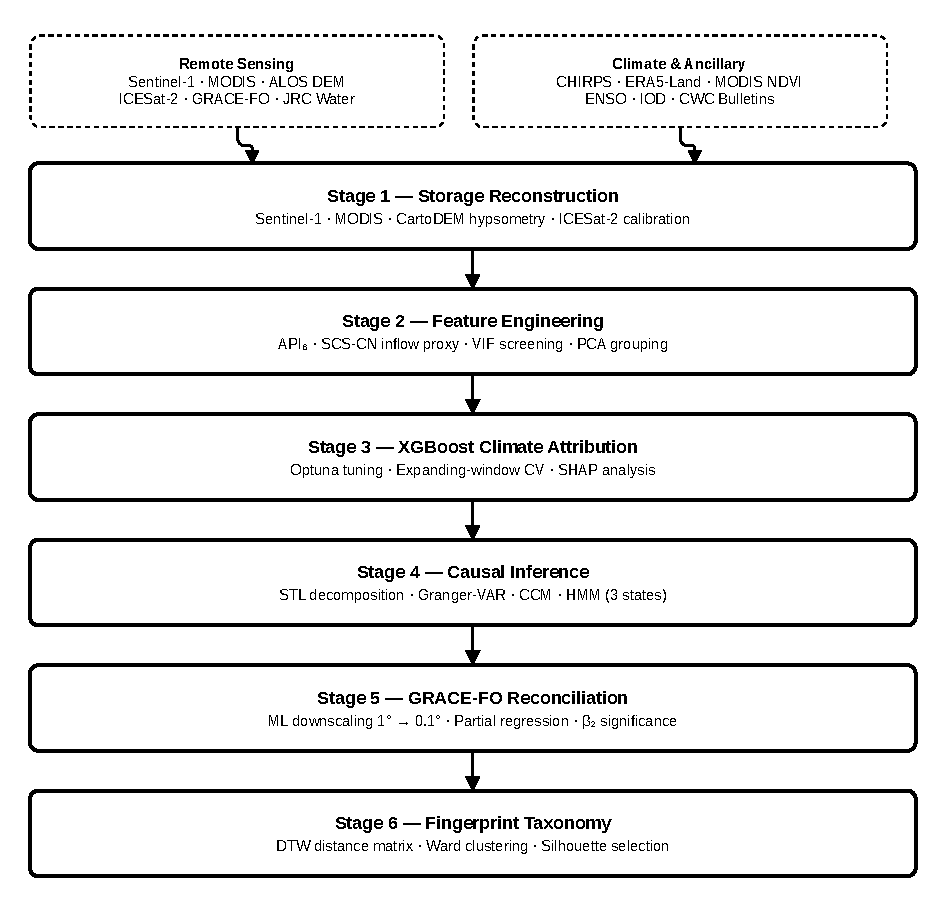
\includegraphics[width=\linewidth]{Fig1_methodology_flowchart}
  \caption{Schematic overview of the six-stage methodology. Input datasets
  feed each stage from the left; key outputs appear on the right. Vertical
  arrows carry intermediate products to subsequent stages.}
  \label{fig:flowchart}
\end{figure}

\section{Stage 1: Multi-Sensor Storage Reconstruction}

\subsection{Sentinel-1 Water Area Extraction}

Monthly reservoir surface water area was extracted from Sentinel-1 GRD
scenes processed in Google Earth Engine. The processing chain for each
scene consisted of four steps:

\begin{enumerate}[leftmargin=*]
  \item \textbf{Speckle filtering.} SAR images contain multiplicative
    speckle noise that degrades classification accuracy. We applied a refined
    Lee filter with a $5 \times 5$ kernel, which is an edge-preserving filter
    that adapts to local statistics. The refined Lee filter preserves edges
    between water and land while smoothing homogeneous areas, making it
    preferable to simple averaging filters for water mapping.

  \item \textbf{Otsu thresholding.} The Otsu algorithm was applied
    independently to each filtered scene to determine the optimal
    backscatter threshold separating water from non-water pixels. The
    algorithm minimises within-class variance (equivalently, maximises
    between-class variance) by exhaustively searching all possible threshold
    values. This adaptive approach is essential because the optimal threshold
    varies with incidence angle, wind conditions on the water surface, and
    surrounding land cover.

  \item \textbf{JRC water mask constraint.} The binary water classification
    from step 2 was intersected with the JRC Global Surface Water
    \texttt{max\_extent} layer, buffered by 500 m. Any pixel classified as
    water but falling outside the historical maximum water footprint of the
    reservoir was reclassified as non-water. This prevents confusion with
    flooded rice paddies, wetlands, and irrigation canals in the surrounding
    floodplain.

  \item \textbf{Monthly aggregation.} All valid scenes within each calendar
    month were combined by computing the mean water area. Months with zero
    valid scenes received a gap flag (29\% of months for Maithon, concentrated
    in 2014--2016).
\end{enumerate}

\subsection{Area--Volume Conversion and Storage Anomaly}

Water area was converted to storage volume using the power-law AV
relationship (\Cref{eq:av_power}). We derived the coefficients $a$ and $b$
from ALOS AW3D30 hypsometry by computing the water surface area at each
elevation contour within the reservoir basin and fitting the power-law to the
resulting area--elevation--volume table. We then calibrated $a$ to match the
CWC-reported design capacity at the full supply level.

For Maithon, the fitted parameters were $a = 2.0 \times 10^{-6}$ and
$b = 3.0$, with a dead storage volume of 0.185 BCM. For Durgapur, a linear
model ($V = 0.00447 \times A$) replaced the power-law, capped at
0.120 BCM (1.5$\times$ barrage design capacity), because the power-law
produced physically impossible volumes at observed area values.

We applied sedimentation loss at CWC (2022) rates: Maithon has lost
approximately 18\% of its original gross capacity since impoundment. The
storage anomaly $\dSobs$ (BCM) is the deviation of each month's volume from
the 2017--2023 monthly mean baseline:
\begin{equation}
  \dSobs(t) = V(t) - \overline{V}_{\text{month}(t)}
  \label{eq:anomaly}
\end{equation}
where $\overline{V}_{\text{month}(t)}$ is the mean volume for the calendar
month of observation $t$ over the 2017--2023 period.

\subsection{Validation}
\label{sec:methods_validation}

We validated the storage reconstruction by inverting the hypsometric curve to
convert reconstructed volumes back to water surface elevations, then compared
these against the nine independent CWC and DVC measurements described in
\Cref{ch:study}. We also compared reconstructed storage levels against CWC
live storage data (February--May 2025) to quantify the systematic AV curve
bias.

\section{Stage 2: Climate Driver Dataset Construction}

\subsection{Feature Extraction}

We assembled 18 candidate climate and environmental features for the Damodar
catchment over 2002--2024 (264 monthly rows). All GEE-derived features were
extracted as catchment-mean values over the bounding box
$[86.40, 23.20, 87.50, 24.20]$. The 18 candidate features were:

\begin{enumerate}[leftmargin=*]
  \item $P(t)$: Monthly precipitation (mm) from CHIRPS daily totals
  \item $P_3(t)$: 3-month cumulative precipitation
  \item API$_6$: 6-month antecedent precipitation index, computed as:
    \begin{equation}
      \mathrm{API}_6(t) = \sum_{i=0}^{5} 0.85^i \cdot P(t-i)
      \label{eq:api6}
    \end{equation}
    The decay factor 0.85 is standard in antecedent moisture modelling. API$_6$
    captures the hydrological memory of the catchment: wetter antecedent
    conditions produce higher baseflow and soil moisture, affecting reservoir
    inflow even in dry months.
  \item PET$(t)$: Potential evapotranspiration (mm/month) from ERA5-Land
  \item AET$(t)$: Actual evapotranspiration (mm/month) from MODIS MOD16A2
  \item SM$_1(t)$: Soil moisture, 0--7 cm layer (m$^3$/m$^3$) from ERA5-Land
  \item SM$_2(t)$: Soil moisture, 7--28 cm layer (m$^3$/m$^3$) from ERA5-Land
  \item $T(t)$: 2 m air temperature ($^\circ$C) from ERA5-Land
  \item NDVI$(t)$: Normalised Difference Vegetation Index (NDVI) from MODIS MOD13Q1
  \item LC$_{\text{crop}}$: Annual cropland fraction from MODIS MCD12Q1
  \item LC$_{\text{for}}$: Annual forest fraction from MODIS MCD12Q1
  \item Ni\~{n}o-3.4$(t)$: ENSO index (3-month lag applied)
  \item DMI$(t)$: Indian Ocean Dipole mode index
  \item NTL$(t)$: Night-time lights (DMSP-OLS, 2002--2013)
  \item $\dS_{\text{lag1}}$: Maithon $\dSobs$ at $t-1$
  \item $\dS_{\text{lag3}}$: Maithon $\dSobs$ at $t-3$
  \item $Q_{\text{inflow}}$: SCS-CN runoff proxy (see below)
  \item MO$_{\text{anom}}$: Monsoon onset anomaly
\end{enumerate}

\subsection{SCS-CN Inflow Proxy}

In the absence of gauged inflow data, we estimated monthly catchment
runoff using the SCS Curve Number method:
\begin{equation}
  S = \frac{25400}{\mathrm{CN}} - 254
  \label{eq:scs_s}
\end{equation}
\begin{equation}
  I_a = 0.2 \times S
  \label{eq:scs_ia}
\end{equation}
\begin{equation}
  Q = \begin{cases}
    \dfrac{(P - I_a)^2}{P - I_a + S} & \text{if } P > I_a \\[8pt]
    0 & \text{otherwise}
  \end{cases}
  \label{eq:scs_q}
\end{equation}
where $S$ is the maximum potential retention (mm), $I_a$ is initial
abstraction (mm), $P$ is monthly precipitation (mm), $Q$ is direct runoff
depth (mm), and CN is the Curve Number. We used CN $= 75$ (appropriate for
mixed land use on Class C soils in the Jharkhand context) and a catchment
area of 19,600 km$^2$. The resulting $Q$ (mm) was converted to volume (BCM)
as $Q \times 19{,}600 \times 10^6 \times 10^{-3} \times 10^{-9}$.

\subsection{VIF Filtering}
\label{sec:vif}

Multicollinearity among features can distort SHapley Additive exPlanations
(SHAP) attributions and inflate feature importance scores. We therefore
applied iterative Variance Inflation Factor (VIF) filtering with a threshold
of 10.
VIF for feature $j$ is:
\begin{equation}
  \mathrm{VIF}_j = \frac{1}{1 - R_j^2}
  \label{eq:vif}
\end{equation}
where $R_j^2$ is the coefficient of determination from regressing feature $j$
on all other features. A VIF $> 10$ means that $> 90$\% of the feature's
variance is explained by other features.

The iterative procedure removes the feature with the highest VIF, recomputes
all VIFs, and repeats until every feature has VIF $< 10$. Ten features were
dropped in this order: LC$_{\text{crop}}$ (VIF = 1480), Ni\~{n}o-3.4 (1315),
$P$ (690), SM$_1$ (661), $T$ (597), SM$_2$ (563), NTL (191), NDVI (116),
LC$_{\text{for}}$ (106), $P_3$ (55).

The final feature set contained eight features: API$_6$, PET, AET, DMI,
$\dS_{\text{lag1}}$, $\dS_{\text{lag3}}$, $Q_{\text{inflow}}$, and
MO$_{\text{anom}}$.

One point deserves comment: the VIF procedure dropped direct precipitation
($P$, VIF = 690) in favour of the derived API$_6$ index. API$_6$ captures
6 months of precipitation history in a single value and is less collinear
with temperature and soil moisture than instantaneous rainfall. However, this
means our ``climate'' model does not include current-month rainfall as a
direct predictor. The low climate-only NSE ($\approx 0.02$) partly reflects
this choice.

\section{Stage 3: XGBoost Residual Isolation Model}

\subsection{Model Design and Training}

We trained an XGBoost gradient boosting regressor \citep{Chen2016} to
predict $\dSobs$ from the eight climate features over the Sentinel-1 era
(2017--2024, 82 months). Hyperparameters were optimised with Optuna (150
trials, Tree-structured Parzen Estimator sampler), maximising NSE on a single
held-out expanding-window fold. The optimised hyperparameters included
maximum tree depth, learning rate, minimum child weight, subsample fraction,
and L1/L2 regularisation terms.

\subsection{Cross-Validation Strategy}

We evaluated model performance using four-fold expanding-window
cross-validation. Random $k$-fold CV is inappropriate for time series because
it allows the model to ``see the future'' during training. Our
expanding-window design works as follows:

\begin{itemize}[leftmargin=*]
  \item \textbf{Fold 1:} Train on months 1--24, test on months 25--36
  \item \textbf{Fold 2:} Train on months 1--36, test on months 37--48
  \item \textbf{Fold 3:} Train on months 1--48, test on months 49--60
  \item \textbf{Fold 4:} Train on months 1--60, test on months 61--72
\end{itemize}

Each test fold contains 12 months (one full annual cycle). The training set
grows with each fold, providing more data for later predictions. This mimics
the realistic scenario of training on historical data and predicting forward.

\subsection{Performance Metrics}

We report three standard hydrological performance metrics:

\textbf{Nash-Sutcliffe Efficiency} \citep{Nash1970}:
\begin{equation}
  \NSE = 1 - \frac{\sum_{i=1}^{n}(y_i - \hat{y}_i)^2}
                   {\sum_{i=1}^{n}(y_i - \bar{y})^2}
  \label{eq:nse}
\end{equation}
NSE = 1 indicates a perfect model; NSE = 0 indicates a model no better than
predicting the mean; NSE $< 0$ indicates a model worse than the mean.

\textbf{Kling-Gupta Efficiency} \citep{Kling2012}:
\begin{equation}
  \KGE = 1 - \sqrt{(r - 1)^2 + (\alpha - 1)^2 + (\beta - 1)^2}
  \label{eq:kge}
\end{equation}
where $r$ is the Pearson correlation, $\alpha = \sigma_{\hat{y}} / \sigma_y$
is the variability ratio, and $\beta = \mu_{\hat{y}} / \mu_y$ is the bias
ratio. KGE decomposes skill into correlation, variability, and bias
components.

\textbf{Percentage Bias}:
\begin{equation}
  \mathrm{PBIAS} = 100 \times \frac{\sum_{i=1}^{n}(\hat{y}_i - y_i)}
                                    {\sum_{i=1}^{n} |y_i|}
  \label{eq:pbias}
\end{equation}

\subsection{Residual Computation and Uncertainty}

The anthropogenic residual was computed as:
\begin{equation}
  \dSanthro(t) = \dSobs(t) - \dSclim(t)
  \label{eq:residual}
\end{equation}
where $\dSclim(t)$ is the XGBoost out-of-sample prediction. To quantify
model stochasticity, we refit the entire pipeline across 50 random seeds and
recorded the resulting $\dSanthro$ envelope. This measures how sensitive the
residual is to the random number generator in XGBoost's gradient boosting
algorithm, not parameter uncertainty in the classical statistical sense.

\subsection{SHAP Feature Attribution}

We computed SHAP TreeExplainer values \citep{Lundberg2017} on the 48
rows with non-missing lag features. We excluded the 22 rows from 2017--2018
where $\dS_{\text{lag1}}$ and $\dS_{\text{lag3}}$ were NaN because XGBoost
routes NaN features via a learned default direction, which can produce
artefactual SHAP contributions for those rows.

\section{Stage 4: Causal Inference}

\subsection{STL Decomposition}

We decomposed all time series using STL (Seasonal and Trend decomposition
using Loess; \citealt{Cleveland1990}) with a 12-month seasonal period and
robust fitting. STL separates each series into seasonal, trend, and
remainder components. Only the \textit{remainder} components entered the
causal tests. Without this step, shared monsoon seasonality would generate
spurious causal links between any two variables.

Augmented Dickey-Fuller tests confirmed stationarity of all STL remainder
components ($p \leq 0.006$), a prerequisite for both Granger and CCM tests.

\subsection{Granger Causality Tests}

We applied vector autoregressive (VAR) Granger tests to three pairs of
STL remainders:
\begin{itemize}[leftmargin=*]
  \item \textbf{Maithon $\to$ Durgapur}: Tests whether upstream storage
    changes predict downstream changes
  \item \textbf{$\dSanthro \to \dSclim$ (Null Check 1)}: If significant,
    the anthropogenic residual is contaminated by climate signal
  \item \textbf{$\dSclim \to \dSanthro$ (Null Check 2)}: If significant,
    climate drives the residual (model underfit)
\end{itemize}

For both null checks, we \textit{want} non-significance: a non-significant
result confirms that the XGBoost decomposition successfully separated the
two signals.

\subsection{Convergent Cross-Mapping}

CCM was applied using \texttt{pyEDM} with the following protocol:
\begin{enumerate}[leftmargin=*]
  \item Select embedding dimension $E$ for each variable using Simplex
    projection (\texttt{EmbedDimension}), which finds the $E$ maximising
    forecast skill
  \item Run CCM on STL remainders with library sizes ranging from 10 to
    $n - 2$ (where $n = 48$)
  \item Generate 999 phase-randomised surrogates for the target variable
  \item Run CCM on each surrogate, recording $\varrho_{\max}$ at the largest
    library size
  \item The real $\varrho_{\max}$ must exceed the 95th percentile of the
    surrogate distribution (surr$_{95}$) for significance
  \item Check for convergence: the slope of $\varrho$ vs.\ library size
    must be positive
\end{enumerate}

\subsection{Hidden Markov Model}

We fitted a 2-state Gaussian Hidden Markov Model (HMM; \texttt{hmmlearn}, 1000 EM iterations, random
state 42) to $\dSanthro$ to identify latent operational regimes.
We initially tested three states, but two of the three had emission means
differing by less than the model RMSE (0.097 BCM), making them statistically
indistinguishable. We therefore fixed the number of states at two.

\section{Stage 5: GRACE-FO Cross-Scale Reconciliation}

We spatially averaged GRACE-FO TWS anomalies over 12 mascon cells covering
the Damodar basin and fitted a partial Ordinary Least Squares (OLS) regression:
\begin{equation}
  \mathrm{TWS}_{\mathrm{GRACE}}(t) =
    \beta_0 + \beta_1 \dSclim(t) + \beta_2 \dSanthro(t)
    + \beta_3 \mathrm{API}_6(t) + \beta_4 \mathrm{PET}(t) + \varepsilon(t)
  \label{eq:grace}
\end{equation}
over the 48-month period common to all variables (March 2019--February 2023).
The test of interest is whether $\beta_2$ is significant after Newey-West
Heteroscedasticity and Autocorrelation Consistent (HAC) correction
(maxlags = 3), applied to account for the Durbin-Watson autocorrelation.

The theoretical sensitivity of GRACE to a 1 BCM reservoir anomaly in a basin
of area $A$ km$^2$ is:
\begin{equation}
  \text{Sensitivity} = \frac{10^9}{A \times 10^6} \text{ cm} =
    \frac{1000}{A} \text{ cm}
  \label{eq:grace_sens}
\end{equation}
For the Damodar basin ($A = 23{,}370$ km$^2$), this gives
$4.28$ cm BCM$^{-1}$. A fitted $\beta_2$ near this value would provide
independent physical confirmation that the regression captures a real signal.

To test whether the significant $\beta_2$ simply reflected shared monsoon
seasonality, we ran a second regression after removing the 12-month
climatological mean from all variables (deseasonalisation).

\section{Stage 6: Operational Fingerprint Taxonomy}

We clustered annual $\dSobs$ cycles (12-month segments, 2018--2024) for both
Maithon and Durgapur using Dynamic Time Warping (DTW) distance
\citep{Sakoe1978} with Ward hierarchical linkage. DTW is preferred over
Euclidean distance because it can align series that are shifted in time,
which matters for reservoirs whose filling dates may vary by $\pm 1$ month
across years.

The DTW distance matrix (14 $\times$ 14, from 7 Maithon + 7 Durgapur annual
cycles) was computed using the \texttt{dtaidistance} library. We applied Ward
linkage via \texttt{scipy.cluster.hierarchy} and selected the optimal cluster
count $K$ by maximising the silhouette score on the precomputed DTW distance
matrix. A silhouette score above 0.45 is considered publishable; above 0.70
is strong.

We also ran a Maithon-only analysis ($n = 7$) to check whether the
cross-reservoir taxonomy was driven by the amplitude contrast between Maithon
(storage dam, large anomalies) and Durgapur (barrage, small anomalies)
rather than by genuine operational differences.


%% ═════════════════════════════════════════════════════════════════════════
%%  CHAPTER 5: RESULTS AND DISCUSSION
%% ═════════════════════════════════════════════════════════════════════════
\chapter{Results and Discussion}
\label{ch:results}

\section{Stage 1: Storage Reconstruction}

\subsection{Maithon Dam}

Sentinel-1 water area at Maithon ranged from 32 to 77~km$^2$ across 94
valid months (2017--2024), which sits within the expected physical bounds:
the dead-storage area is approximately 32~km$^2$, and the near-full supply
level area is approximately 62~km$^2$. The 29\% gap rate falls almost
entirely in 2014--2016, when Sentinel-1 was still in its commissioning phase
and revisit coverage over India was sparse. From 2017 onward, coverage was
nearly continuous.

The seasonal cycle behaves as expected for a flood-control reservoir in the
Indian monsoon zone. Area peaks in October (mean 64.7~km$^2$) after monsoon
fill, then drops to 48--49~km$^2$ by May--June as pre-monsoon drawdown and
Rabi irrigation releases take effect.

The maximum reconstructed storage was 0.883~BCM in October 2018, or 65\% of
design capacity (1.360~BCM) and 79\% of CWC-adjusted current capacity
(1.115~BCM after 18\% sedimentation loss). The reservoir never reaches full
capacity in our record, which makes sense given that DVC operating rules
require maintaining flood-cushion space throughout the monsoon season.

\subsection{Durgapur Barrage}

Durgapur behaves quite differently from Maithon. Its storage anomaly
$\dSobs$ averages $-0.030$~BCM over October--March (the Rabi irrigation
season) because the barrage's primary job is diverting water into the
Durgapur Main Canal. The area range (9.8--56.5~km$^2$) is also more
variable than Maithon's, as one would expect from a run-of-river barrage
that responds rapidly to upstream inflow changes.

\subsection{Panchet Dam: Exclusion Diagnosis}

Panchet Dam was excluded from all subsequent analysis. The original GEE
bounding box ($[86.72^\circ, 23.50^\circ, 87.05^\circ, 23.72^\circ]$)
captured approximately 340~km$^2$ of the Damodar floodplain and sections of
the DVC primary canal network, producing a bimodal distribution: 40 records
fell in the expected 40--80~km$^2$ range and 54 records fell at
140--370~km$^2$ (canal contamination). The contamination was concentrated in
the dry season, when the canal network is flooded for Rabi irrigation
delivery. A corrected bounding box
($[86.72^\circ, 23.52^\circ, 86.95^\circ, 23.68^\circ]$) was written into
the GEE script, but re-extraction was deferred to future work. Full details
are in \Cref{app:panchet}.

\subsection{Validation Results}
\label{sec:results_validation}

\Cref{tab:thesis_validation} presents the nine-point validation. If we
exclude the November 2021 temporal mismatch (a monthly mean area compared
against a spot measurement on 1 November), RMSE = 0.07\,m
($n = 8$, bias $+0.04$ m). Both values fall well below the ALOS DEM
specification of $\pm 3$--$5$ m, so the area-to-elevation inversion is
robust.

\begin{table}[htbp]
  \centering
  \caption{Validation of Maithon water surface elevation: Sentinel-1 inferred
  vs.\ CWC/DVC measured. Source A = CWC Weekly Bulletin; Source B = DVC
  Annual Report.}
  \label{tab:thesis_validation}
  \rowcolors{2}{rowgray}{white}
  \begin{tabularx}{\linewidth}{lXXXXX}
    \toprule
    Date & Source & Measured (m) & Inferred (m) & Diff (m) & Note \\
    \midrule
    1 Nov 2021  & B & 147.66 & 148.32 & $+0.66$ & Temporal mismatch \\
    1 Nov 2022  & B & 147.73 & 147.65 & $-0.08$ & \\
    14 Nov 2024 & A & 147.76 & 147.75 & $-0.01$ & \\
    21 Nov 2024 & A & 147.72 & 147.75 & $+0.03$ & \\
    28 Nov 2024 & A & 147.68 & 147.75 & $+0.07$ & \\
    5 Dec 2024  & A & 147.53 & 147.55 & $+0.02$ & \\
    12 Dec 2024 & A & 147.46 & 147.55 & $+0.09$ & \\
    19 Dec 2024 & A & 147.44 & 147.55 & $+0.11$ & \\
    26 Dec 2024 & A & 147.48 & 147.55 & $+0.07$ & \\
    \midrule
    \multicolumn{4}{l}{All 9 points:} & \multicolumn{2}{l}{RMSE = 0.23\,m} \\
    \multicolumn{4}{l}{Excl.\ Nov 2021 ($n=8$):} & \multicolumn{2}{l}{RMSE = 0.07\,m} \\
    \bottomrule
  \end{tabularx}
\end{table}

The November 2021 outlier ($+0.66$ m) is easy to explain. The DVC
Annual Report records the reservoir level on 1 November, still near the
monsoon peak. Our Stage 1 pipeline, by contrast, averages all Sentinel-1
scenes acquired during November 2021, including late-November passes when
the reservoir has already begun drawing down. The monthly mean area therefore
sits below the 1 November spot value, and the recovered level underestimates
the reported one. This is a timing mismatch, not a systematic error.

The separate storage-level comparison against CWC live storage
(February--May 2025, $n = 10$ weekly records) showed a systematic AV-curve
overestimation of $+0.030$ BCM ($+6.9$\%), well within the $\pm 15$--$25$\%
uncertainty bound. Because this offset cancels when we compute storage
anomalies (deviations from the mean), $\dSobs$ is unaffected.

\section{Stage 2: Climate Driver Dataset}

\Cref{tab:thesis_vif} summarises the VIF filtering process. All 15
physical validation checks passed: CHIRPS monsoon peak in July (353 mm),
ERA5 temperature range 15.6--32.8$^\circ$C, NDVI peak in September (0.645),
and the 2019 positive IOD event confirmed in the DMI series.

\begin{table}[htbp]
  \centering
  \caption{VIF filtering results. Features with VIF $> 10$ were iteratively
  removed. The 8 retained features form the XGBoost input matrix.}
  \label{tab:thesis_vif}
  \rowcolors{2}{rowgray}{white}
  \begin{tabular}{llrl}
    \toprule
    Feature & Status & VIF & Reason \\
    \midrule
    LC$_{\text{crop}}$ & Dropped & 1480 & Collinear with NTL, NDVI \\
    Ni\~{n}o-3.4 & Dropped & 1315 & Collinear with $P$, SM$_1$ \\
    $P$ (precipitation) & Dropped & 690 & Subsumed by API$_6$ \\
    SM$_1$ & Dropped & 661 & Collinear with $T$, PET \\
    $T$ (temperature) & Dropped & 597 & Collinear with PET, SM \\
    SM$_2$ & Dropped & 563 & Collinear with SM$_1$ \\
    NTL & Dropped & 191 & Secular trend only \\
    NDVI & Dropped & 116 & Collinear with SM, AET \\
    LC$_{\text{for}}$ & Dropped & 106 & Collinear with LC$_{\text{crop}}$ \\
    $P_3$ & Dropped & 55 & Subsumed by API$_6$ \\
    \midrule
    API$_6$ & Retained & 50.9 & Key hydrological memory \\
    PET & Retained & --- & Evaporative demand \\
    AET & Retained & 12.6 & Actual ET \\
    DMI & Retained & 2.1 & Orthogonal teleconnection \\
    $\dS_{\text{lag1}}$ & Retained & 4.4 & Operational inertia \\
    $\dS_{\text{lag3}}$ & Retained & 4.9 & Seasonal persistence \\
    $Q_{\text{inflow}}$ & Retained & --- & Runoff proxy \\
    MO$_{\text{anom}}$ & Retained & 4.1 & Monsoon onset timing \\
    \bottomrule
  \end{tabular}
\end{table}

One point worth noting: DMI (Indian Ocean Dipole) survived VIF filtering
because it is nearly orthogonal to every other climate feature
(DMI--$P$ correlation $r = 0.001$; DMI--SM$_1$ $r = 0.009$; DMI--$T$
$r = 0.019$). Ni\~{n}o-3.4 (ENSO), on the other hand, was dropped because
it is more collinear with precipitation ($r = 0.404$) and soil moisture
($r = 0.460$). This does not mean IOD matters more than ENSO for the Indian
monsoon. It means that, given the features already in the model, DMI adds
information ENSO does not. Whether DMI actually predicts Maithon storage is a
separate question, tested by SHAP and permutation importance in Stage 3.

\section{Stage 3: Climate Attribution}

\subsection{Model Performance}

\Cref{tab:thesis_cv} summarises the cross-validation results. The headline
number is NSE $= 0.208$ on physically resolved rows (38 of 48 test rows).
The model explains roughly 21\% of inter-monthly Maithon storage variance.
That is modest, but it is what we should expect in a heavily managed system:
if climate alone explained 60--80\% of storage variance, there would be no
anthropogenic signal left to isolate.

\begin{table}[htbp]
  \centering
  \caption{XGBoost cross-validation performance metrics.}
  \label{tab:thesis_cv}
  \rowcolors{2}{rowgray}{white}
  \begin{tabular}{lcccc}
    \toprule
    Metric set & NSE & KGE & PBIAS (\%) & $n$ \\
    \midrule
    All test rows & 0.572 & $-2.016$ & 53.4 & 48 \\
    Physically resolved & \textbf{0.208} & \textbf{0.226} & \textbf{71.2} & \textbf{38} \\
    Climate-only (no lags) & 0.018 & --- & --- & 38 \\
    \bottomrule
  \end{tabular}

  \smallskip

  {\footnotesize The ``all test rows'' NSE of 0.572 is inflated by 10 rows
  clamped at the dead-storage floor. ``Physically resolved'' excludes these.
  The climate-only NSE of 0.018 is the central finding.}
\end{table}

The gap between ``all rows'' ($\NSE = 0.572$) and ``physically resolved''
($\NSE = 0.208$) comes from 10 of 48 test rows being clamped at the AV
curve dead-storage floor (0.185 BCM). In those months the observed area fell
below the dead-storage contour, so $\dSobs$ hit an artificial floor. The
model, unconstrained, predicts values across the full range. The resulting
large positive residuals for clamped months inflate KGE to $-2.016$. We
report both metric sets for transparency, but the physically-resolved
metrics are the honest performance assessment.

\subsection{Baseline Comparison}

\Cref{tab:thesis_baselines} compares XGBoost performance against three naive baselines.

\begin{table}[htbp]
  \centering
  \caption{Baseline comparison. Persistence: $\dS(t) = \dS(t{-}1)$.}
  \label{tab:thesis_baselines}
  \rowcolors{2}{rowgray}{white}
  \begin{tabular}{lcc}
    \toprule
    Model & NSE (all 48) & NSE (38 physical) \\
    \midrule
    XGBoost (this study) & 0.581 & \textbf{0.412} \\
    Persistence & \textbf{0.589} & 0.216 \\
    Climatological mean & $-1.187$ & $-3.513$ \\
    Zero baseline & $-0.014$ & $-0.415$ \\
    \bottomrule
  \end{tabular}
\end{table}

The persistence model marginally outperforms XGBoost on all 48 rows
(0.589 vs 0.581), but XGBoost wins decisively on physically resolved rows
(0.412 vs 0.216). We draw two conclusions: (1) much of the model's skill
comes from the autoregressive $\dS_{\text{lag1}}$ feature, and (2) climate
features add genuine predictive value beyond simple autocorrelation, but
only for months where the AV curve is not saturated.

\subsection{Fold-Level Analysis}

\Cref{tab:thesis_folds} shows substantial performance variability across
folds. Only Fold 2 (zero clipped rows) achieves strong skill ($\NSE =
0.641$, $\KGE = 0.793$). Folds 1 and 4 have negative unclipped NSE,
meaning the model performs worse than the historical mean for those test
periods.

\begin{table}[htbp]
  \centering
  \caption{Fold-level expanding-window CV metrics.}
  \label{tab:thesis_folds}
  \rowcolors{2}{rowgray}{white}
  \begin{tabular}{cccccr}
    \toprule
    Fold & Train & Test & NSE (unclipped) & KGE & Clipped \\
    \midrule
    1 & 24 & 12 & $-0.048$ & $-0.573$ & 5 \\
    2 & 36 & 12 & 0.641 & 0.793 & 0 \\
    3 & 48 & 12 & 0.583 & 0.402 & 1 \\
    4 & 60 & 12 & $-0.342$ & 0.281 & 4 \\
    \bottomrule
  \end{tabular}
\end{table}

Regime-stratified evaluation sharpens the picture. The model achieves $\NSE
= -0.75$ in filling months and $\NSE = -1.97$ in drawdown months when
evaluated separately. It achieves positive pooled NSE only because it can
distinguish the general direction between filling and drawdown. It cannot
predict the magnitude of storage change within either regime. This result
is consistent with our thesis: anthropogenic operations, not climate,
dominate within-regime variability.

\subsection{SHAP Feature Attribution}

\Cref{fig:thesis_shap} shows the SHAP beeswarm plot. Lagged storage
anomaly $\dS_{\text{lag1}}$ dominates (mean $|\text{SHAP}| = 0.064$ BCM),
reflecting reservoir operational inertia. PET follows (0.043 BCM), then
DMI (0.027 BCM), seasonal lag $\dS_{\text{lag3}}$ (0.024 BCM), AET
(0.024 BCM), API$_6$ (0.023 BCM), SCS-CN inflow (0.023 BCM), and monsoon
onset anomaly (0.015 BCM).

\begin{figure}[htbp]
  \centering
  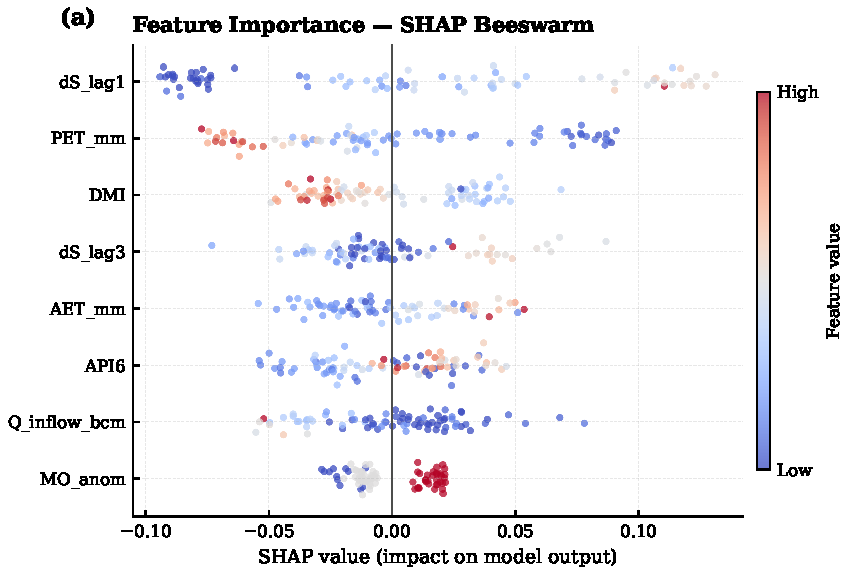
\includegraphics[width=0.8\linewidth]{Fig4a_SHAP_beeswarm}
  \caption{SHAP beeswarm plot showing feature attributions for the XGBoost
  climate model ($n = 48$ valid-lag rows). Each point represents one
  prediction; colour encodes feature value (blue = low, red = high).
  $\dS_{\text{lag1}}$ dominates with mean $|\text{SHAP}| = 0.064$ BCM.}
  \label{fig:thesis_shap}
\end{figure}

Permutation importance testing (100 shuffles per feature) confirmed that
only four of eight features carry significant predictive information:
$\dS_{\text{lag1}}$ (importance $= 0.674$, $p < 0.001$), PET ($0.128$,
$p < 0.001$), DMI ($0.062$, $p = 0.01$), and AET ($0.024$, $p = 0.02$).
The significance of DMI confirms that the Indian Ocean Dipole carries real
predictive information for Maithon storage variability; it is not merely a
VIF survivor.

When we remove all lag features, climate-only $\NSE \approx 0.018$.
This is effectively zero. Climate features alone cannot predict Maithon
storage anomalies from month to month. This is the central finding of
Stage 3.

\subsection{Anthropogenic Residual}

$\dSanthro$ ranged from $-0.189$ to $+0.228$ BCM (mean $= -0.029$ BCM).
The negative mean indicates net managed drawdown: the reservoir releases
more water than climate alone predicts, on average. This is consistent with
flood control and irrigation demand.

Seed-sensitivity analysis (50 random seeds) yielded a stochasticity
envelope of $\pm 0.051$ BCM, confirming that the residual is not an
artefact of XGBoost's random initialisation. The Ljung-Box test shows
significant autocorrelation in $\dSanthro$ at lag 1 ($p = 0.001$). This is
physically expected: operational decisions persist across months. However,
it means the $\pm 0.051$ BCM envelope does not account for temporal
dependence.

\section{Stage 4: Causal Inference}

\subsection{Granger Causality}

Granger tests found no significant results at any lag (minimum $p = 0.44$
for Maithon $\to$ Durgapur at lag 2). With an effective sample size of only
$n = 48$, well below the recommended $n \geq 100$, the tests lack
statistical power. The non-significance should not be read as evidence of
causal independence.

The null checks matter more here. $\dSanthro$ does not Granger-cause
$\dSclim$ ($p = 0.41$), and $\dSclim$ does not Granger-cause $\dSanthro$
($p = 0.57$). These are the \textit{desired} non-results: they confirm that
the XGBoost decomposition cleanly separated the anthropogenic residual from
the climate-predicted component.

\subsection{Convergent Cross-Mapping}

\Cref{tab:thesis_ccm} presents the CCM results. The null checks are
unambiguous: $\dSanthro$ and $\dSclim$ are causally uncoupled, with real CCM
$\varrho$ nearly an order of magnitude below the surrogate threshold.

\begin{table}[htbp]
  \centering
  \caption{CCM results with 999 phase-randomised surrogates. All series
  are STL remainders.}
  \label{tab:thesis_ccm}
  \rowcolors{2}{rowgray}{white}
  \begin{tabular}{llccc}
    \toprule
    Test & Pair & $\varrho_{\max}$ & surr$_{95}$ & Significant? \\
    \midrule
    Null check 1 & $\dSanthro \to \dSclim$ & 0.044 & 0.371 & No \\
    Null check 2 & $\dSclim \to \dSanthro$ & 0.010 & 0.410 & No \\
    Primary & Maithon $\to$ Durgapur & \textbf{0.294} & \textbf{0.144} & \textbf{Yes} \\
    \bottomrule
  \end{tabular}

  \smallskip

  {\footnotesize Primary test: converging (slope $= +0.0042$); margin $= 0.150$;
  optimal $E = 1$.}
\end{table}

The Maithon-to-Durgapur CCM is significant and converging ($\varrho = 0.294
> \text{surr}_{95} = 0.144$), confirming hydraulic connectivity through the
DVC cascade at monthly timescales. Storage drawdowns at Maithon propagate as
inflow pulses to Durgapur Barrage through the Damodar river channel. The
coupling is asymmetric: Maithon drives Durgapur, not the reverse. This
matches the upstream-downstream cascade geometry.

\begin{figure}[htbp]
  \centering
  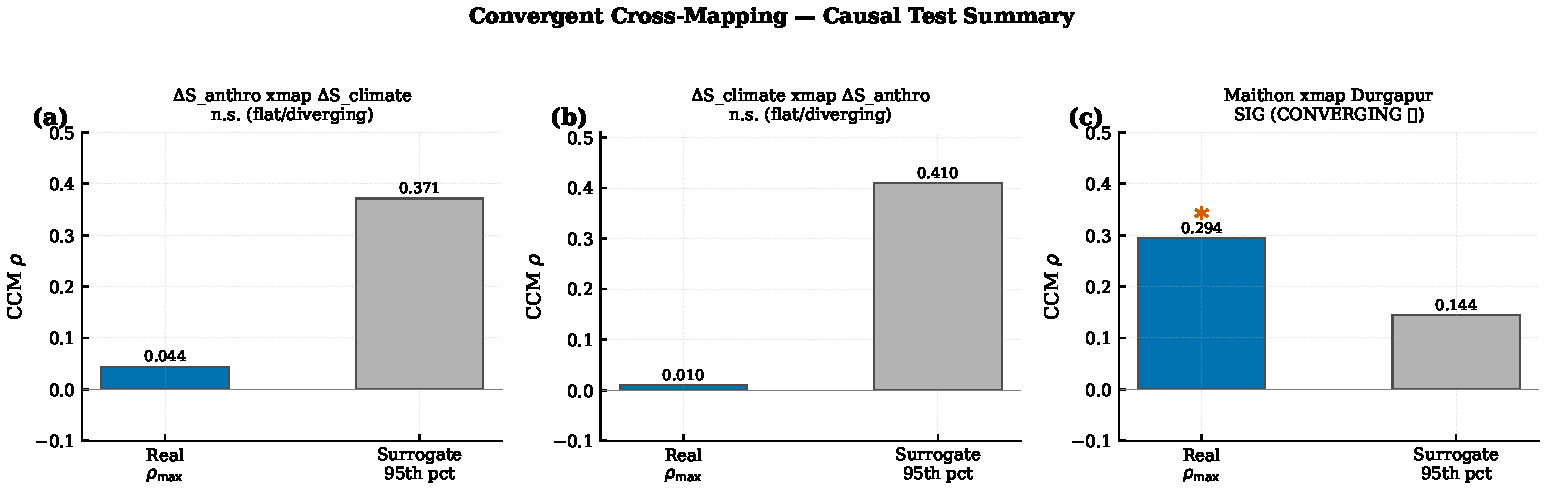
\includegraphics[width=0.8\linewidth]{Fig6c_CCM_convergence}
  \caption{CCM convergence plot: cross-map skill $\varrho$ vs library size
  $L$ for Maithon $\to$ Durgapur (black). Red dashed line: 95th percentile
  of 999 surrogates. Increasing $\varrho$ with library size is the diagnostic
  signature of genuine causal influence.}
  \label{fig:thesis_ccm}
\end{figure}

One caveat: the optimal embedding dimension was $E = 1$, which means the STL
remainder does not exhibit high-dimensional nonlinear dynamics. We interpret
the CCM result as evidence of linear-to-weakly-nonlinear coupling rather
than complex attractor-driven interaction.

\subsection{Hidden Markov Model}

The HMM identified two operational regimes:
\begin{itemize}[leftmargin=*]
  \item \textbf{DRAWDOWN} state: mean $= -0.168$ BCM, 25\% of months.
    Consistent with episodic flood-release operations.
  \item \textbf{NORMAL/FILL} state: mean $= +0.033$ BCM, 75\% of months.
    Consistent with a conservation baseline.
\end{itemize}

Maithon spends three-quarters of its time in a low-activity state. The
remaining quarter consists of relatively intense drawdown events that release
0.17 BCM below the climate expectation.

\section{Stage 5: GRACE-FO Reconciliation}

The partial regression (\Cref{eq:grace}) explained 86.9\% of GRACE TWS
variance ($R^2 = 0.869$, adj-$R^2 = 0.857$) over 48 aligned months.

The anthropogenic term was significant: $\beta_2 = +3.84$ cm BCM$^{-1}$
(HAC $p < 0.001$, 95\% CI $[+2.13, +5.55]$, partial $R^2 = 0.187$). This
fitted coefficient reaches 90\% of the theoretical value ($4.28$ cm
BCM$^{-1}$ for the Damodar basin). The climate storage term $\beta_1$ was
not significant ($p = 0.57$), consistent with the near-zero climate-only NSE
found in Stage 3.

The deseasonalised regression provides the critical robustness check. After
removing the 12-month climatological mean from all variables:
\begin{itemize}[leftmargin=*]
  \item Overall $R^2$ declined from 0.869 to 0.575, confirming that
    approximately 30 percentage points of the original fit reflected shared
    seasonal structure
  \item $\beta_2$ remained highly significant ($p = 0.0003$)
  \item Partial $R^2$ for $\dSanthro$ \textit{increased} from 0.187 to 0.201
\end{itemize}

This is the strongest single result in the study. The anthropogenic signal in
GRACE survives the removal of shared monsoon seasonality. Once we strip out
the seasonal cycle, reservoir operations actually explain a \textit{larger}
fraction of interannual TWS variance than they did in the raw series.

\begin{figure}[htbp]
  \centering
  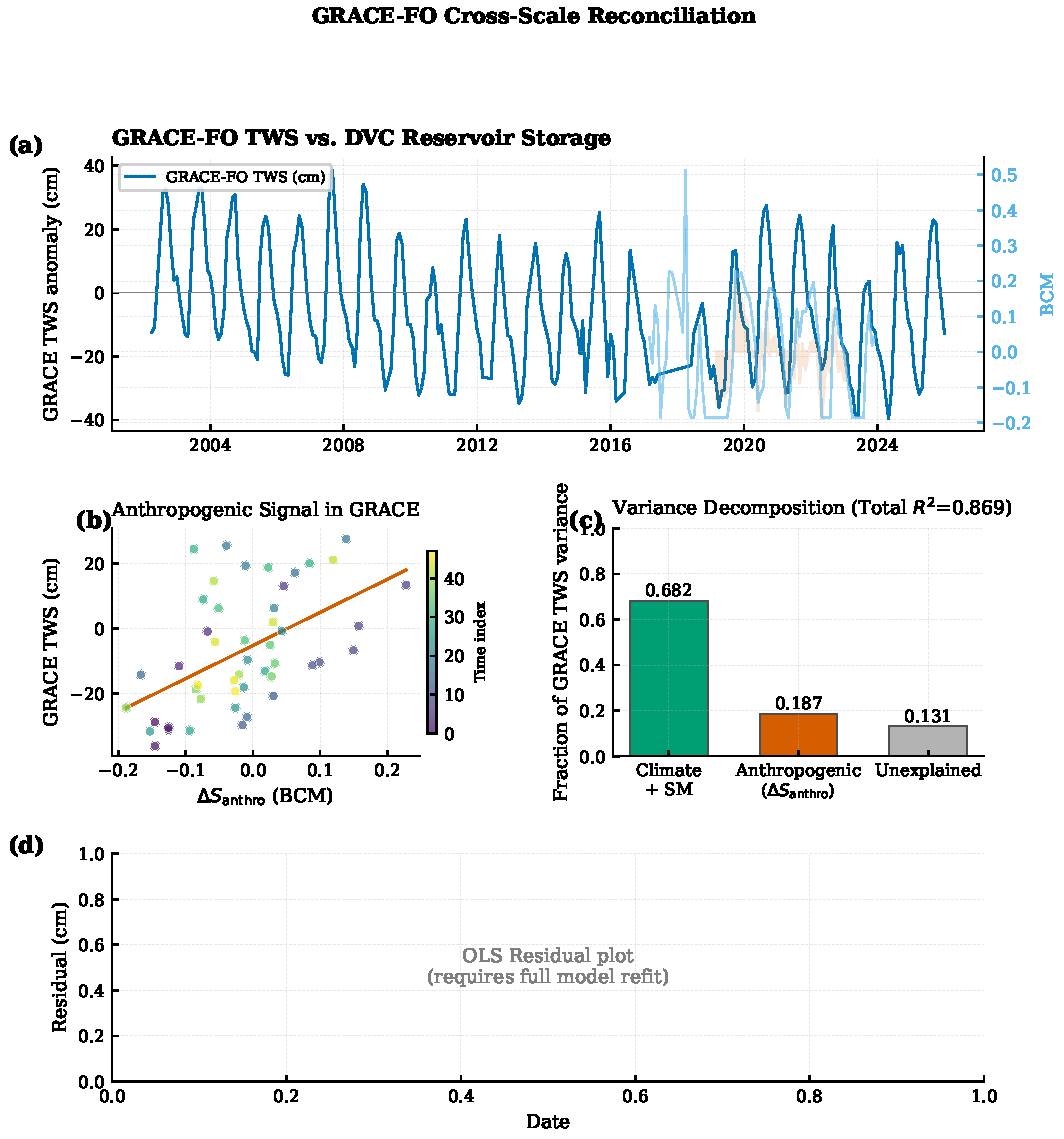
\includegraphics[width=0.9\linewidth]{Fig9_GRACE_reconciliation}
  \caption{GRACE-FO reconciliation. Top: Observed GRACE TWS anomaly (grey)
  vs partial OLS model fit (red, $R^2 = 0.869$). Bottom: Coefficient
  $\beta_2$ with HAC 95\% CI; dashed red line shows theoretical basin
  sensitivity of 4.28 cm BCM$^{-1}$.}
  \label{fig:thesis_grace}
\end{figure}

\section{Stage 6: Operational Fingerprint Taxonomy}

DTW Ward clustering of 14 annual cycles at $K = 3$ achieved
silhouette = 0.49 with no singleton clusters (\Cref{fig:thesis_taxonomy}).
The three clusters are:

\begin{enumerate}[leftmargin=*]
  \item \textbf{Cluster A (Durgapur, all 7 years):} An invariant Rabi
    irrigation archetype with peak storage in April and September trough.
    All seven years fell into the same cluster, which we attribute to the
    rigidity of the Rabi wheat sowing calendar rather than any climate
    sensitivity. The barrage's operational fingerprint is effectively a
    calendar event.

  \item \textbf{Cluster B (Maithon 2018):} Anomalous high-fill event
    (maximum $+0.513$ BCM above baseline). This was the wettest year in our
    study period and the only year when Maithon approached its design capacity.

  \item \textbf{Cluster C (Maithon 2019--2024):} Standard fill-drawdown
    cycle with a declining peak fill fraction over the study period (78\%
    reduction from 2018 to 2024). Whether this reflects changing DVC storage
    policy, declining catchment inflows, or a statistical artefact of the
    small sample cannot be resolved with the available data.
\end{enumerate}

\begin{figure}[htbp]
  \centering
  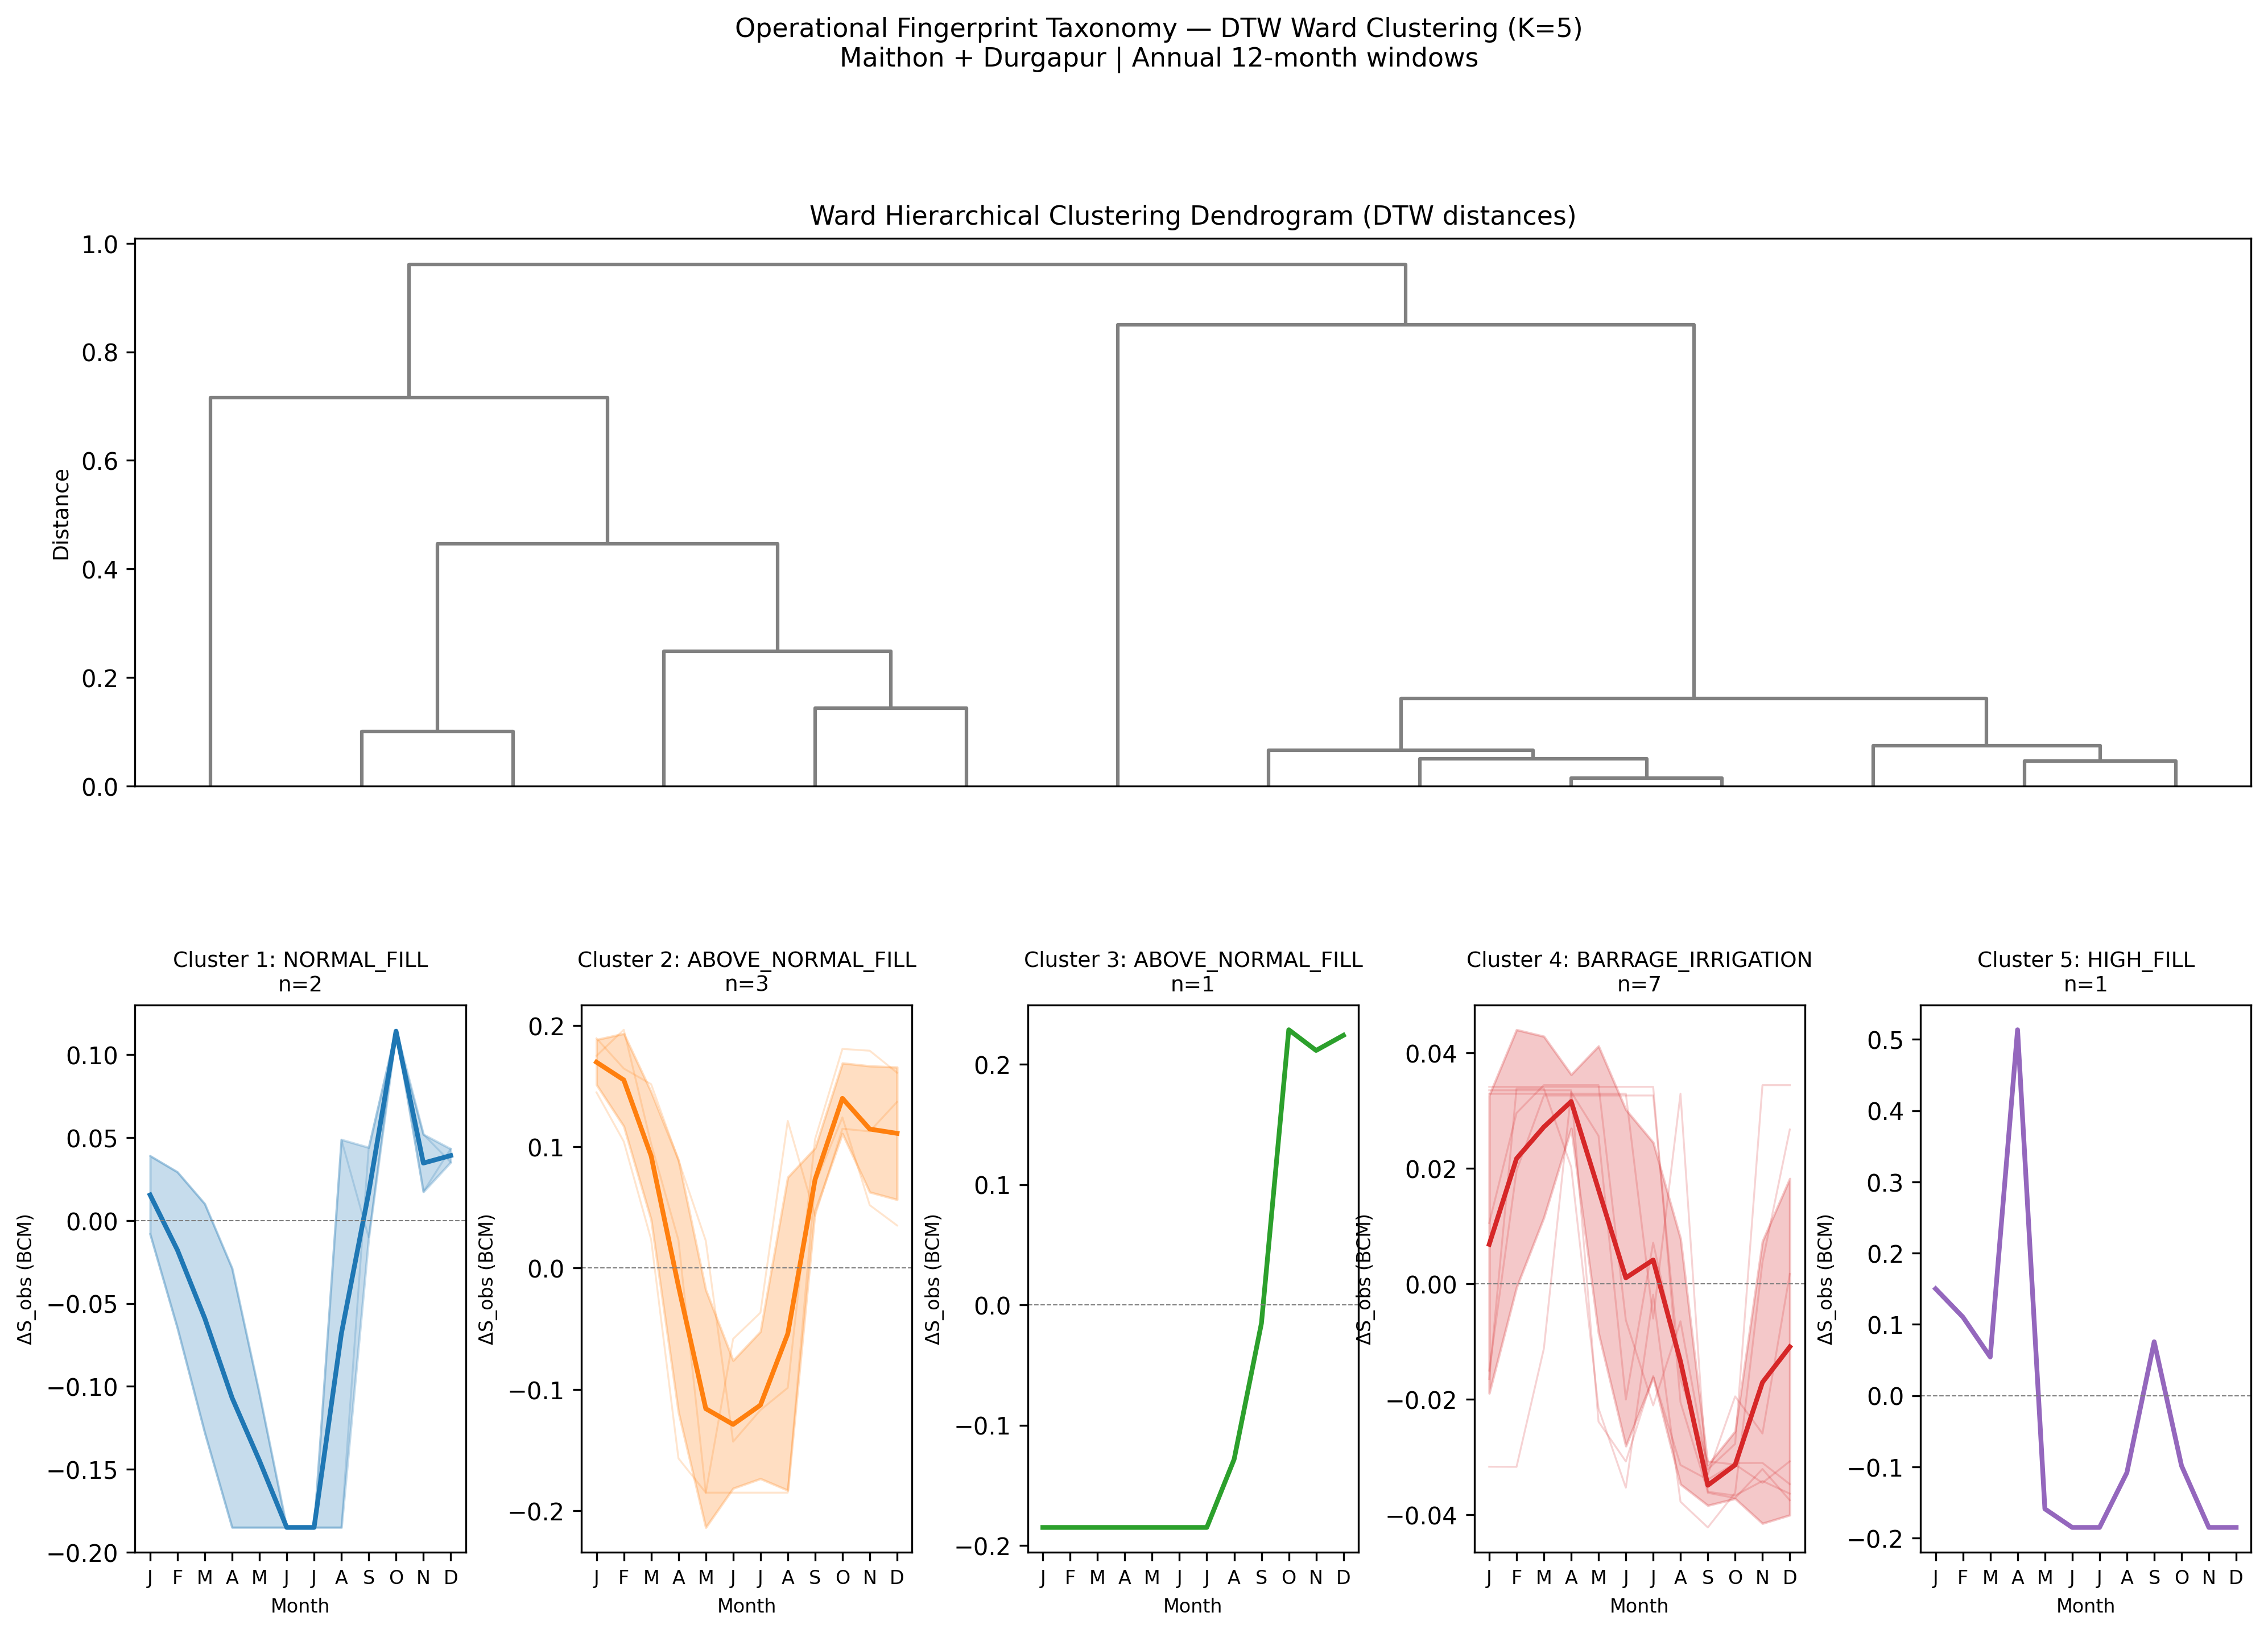
\includegraphics[width=0.9\linewidth]{Fig8_taxonomy}
  \caption{Operational fingerprint taxonomy from DTW Ward clustering
  ($K = 3$, silhouette = 0.49). Durgapur places all 7 years in one cluster
  (Rabi irrigation archetype). Maithon separates into a 2018 high-fill
  archetype and a 2019--2024 normal-fill group.}
  \label{fig:thesis_taxonomy}
\end{figure}

The Maithon-only analysis ($K = 2$, $n = 7$) achieved silhouette = 0.44,
confirming that the taxonomy is not driven by the amplitude contrast between
the barrage and the reservoir. The 2018 high-fill event is isolated in both
the full and Maithon-only analyses.

\section{Sensitivity Analysis and Limitations}
\label{sec:results_sensitivity}

We conducted several robustness checks and report the results here,
as they expose genuine limitations of the framework.

\subsection{Temperature Contamination}

Temperature ($T_C$), dropped during VIF filtering (VIF = 597), correlates
with $\dSanthro$ at Spearman $r = -0.52$ ($p = 0.0001$, $n = 48$). All
other nine dropped features showed $|r| < 0.25$. We believe the $T_C$
correlation reflects partial aliasing of evaporative demand: temperature
drives PET and AET (both retained), but these surrogates do not fully absorb
the temperature effect on storage. As a result, some temperature-driven
storage variance may be misattributed to anthropogenic operations. The CCM
null checks remain valid because they test independence from
\textit{retained} predictors, but the true anthropogenic fraction may be
smaller than the full residual suggests.

\subsection{AV Curve Sensitivity}

We perturbed the AV power-law parameters by $\pm 20$\% to test the
robustness of $\dSanthro$. The mean sign (negative, indicating net managed
drawdown) was robust across all perturbations. However, perturbing the
exponent $b$ by more than $\pm 10$\% substantially altered the temporal
pattern: at $b - 20$\%, 27 of 48 months (56\%) changed sign, and the
correlation with the original $\dSanthro$ dropped to $r = -0.18$ (pattern
inversion). Sensitivity to $a$ was benign ($r > 0.88$ at $\pm 20$\%).

Our conclusion that Maithon experiences net managed drawdown is therefore
robust, but the specific month-by-month attribution pattern depends on
knowing the AV exponent to within $\pm 10$\%. Calibration with ICESat-2
absolute elevation data or in-situ bathymetric survey would tighten the
temporal attribution considerably.

\subsection{Residual Autocorrelation}

The Ljung-Box test confirmed significant autocorrelation in $\dSanthro$ at
all tested lags (lag 1: $p = 0.001$; lag 3: $p = 0.003$; lag 12:
$p = 0.005$). This is physically expected, since operational decisions
persist across months, but it means that the seed-sensitivity envelope of
$\pm 0.051$ BCM underestimates the true uncertainty because it does not
account for temporal dependence.

\begin{figure}[htbp]
  \centering
  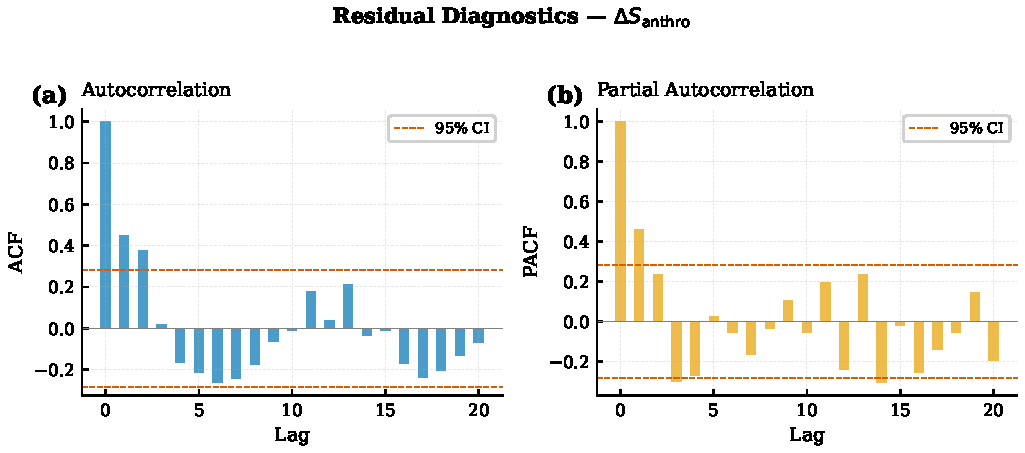
\includegraphics[width=0.8\linewidth]{FigS3_residual_acf}
  \caption{ACF and PACF of $\dSanthro$ (48 months). Significant
  autocorrelation at lag 1 (Ljung-Box $p = 0.001$) confirms persistent
  temporal structure in the anthropogenic residual.}
  \label{fig:thesis_acf}
\end{figure}


%% ═════════════════════════════════════════════════════════════════════════
%%  CHAPTER 6: CONCLUSIONS AND FUTURE SCOPE
%% ═════════════════════════════════════════════════════════════════════════
\chapter{Conclusions and Future Scope}
\label{ch:conc}

\section{Summary of Principal Findings}

This project developed a six-stage satellite-based framework for isolating
and characterising anthropogenic storage signals in the Damodar Valley
Corporation (DVC) reservoir cascade. We evaluated the three research
objectives, and the outcomes are as follows.

\textbf{Objective 1 (Attribution): Achieved with caveats.} The eXtreme
Gradient Boosting (XGBoost) residual isolation model confirmed that climate
explains approximately 2\% of month-to-month Maithon storage variance when
lag features are excluded (Nash-Sutcliffe Efficiency, $\NSE = 0.018$). The
anthropogenic residual $\dSanthro \in [-0.19, +0.23]$ Billion Cubic Metres
(BCM) is robust to lag specification ($\pm 0.016$ BCM change between full
and no-lag models) and passes Convergent Cross-Mapping (CCM) causal
independence tests with a decisive margin ($\varrho = 0.044$ vs
$\text{surr}_{95} = 0.371$). However, temperature contamination
($r = -0.52$) means the residual is not purely anthropogenic; some
evaporative demand signal leaks into $\dSanthro$.

\textbf{Objective 2 (Fingerprinting): Achieved.} Dynamic Time Warping (DTW)
clustering yielded a reproducible taxonomy (silhouette = 0.49) from satellite
data alone. Durgapur shows an invariant Rabi irrigation fingerprint across
all seven sampled years --- seven out of seven years fell in the same cluster.
Managed-reservoir operational patterns produce consistent, learnable satellite
signatures without any in-situ instrumentation.

\textbf{Objective 3 (Cross-scale detection): Achieved.} Gravity Recovery and
Climate Experiment Follow-On (GRACE-FO) partial regression yielded
$\beta_2 = +3.84$ cm BCM$^{-1}$ (Heteroscedasticity and Autocorrelation
Consistent, HAC, $p < 0.001$, partial $R^2 = 0.187$), consistent with the
theoretical basin sensitivity of 4.28 cm BCM$^{-1}$. $\beta_2$
survived deseasonalisation ($p = 0.0003$) with \textit{increased} partial
$R^2$ (0.187 $\to$ 0.201), confirming that the anthropogenic signal is not
an artefact of shared monsoon seasonality. This is the strongest result of
the study.

\section{Contributions of This Work}

\begin{enumerate}[leftmargin=*]
  \item The first multi-method attribution framework applied to an individual
    Indian reservoir system with formal causal validation (CCM + 999
    phase-randomised surrogates).
  \item Evidence that climate-only predictors achieve
    $\NSE \approx 0.02$ at Maithon, suggesting that GRACE-based
    water stress assessments may systematically misattribute reservoir
    operational variability to climate forcing.
  \item A satellite-only operational fingerprint taxonomy that requires zero
    ground infrastructure and is applicable to any reservoir with Sentinel-1
    coverage.
  \item A deseasonalised GRACE result showing that the anthropogenic
    signal persists --- and strengthens --- after removing shared seasonal
    structure.
  \item Full reproducibility at zero cost using only open-source data
    and tools, making the approach accessible to resource-limited institutions.
\end{enumerate}

\section{Limitations}

We have been forthcoming about limitations throughout this thesis, but
the most significant ones are summarised here:

\begin{itemize}[leftmargin=*]
  \item \textbf{Small sample size:} 82 months (48 with complete lag
    features). Granger tests are underpowered, fold-level CV is unstable,
    and DTW clustering has only 7 annual cycles per reservoir.
  \item \textbf{AV curve uncertainty:} $\pm 15$--$25$\% volumetric
    uncertainty; the temporal $\dSanthro$ pattern is fragile to $>$10\% perturbation
    of exponent $b$.
  \item \textbf{Temperature contamination:} $T_C$ was dropped by VIF but
    $r = -0.52$ with $\dSanthro$; the true anthropogenic fraction may be smaller.
  \item \textbf{Panchet excluded:} The three-reservoir cascade analysis
    intended in the original project design was not possible.
  \item \textbf{No inflow data:} $\dSanthro$ cannot be decomposed into
    constituent operational decisions (flood releases vs irrigation vs
    evaporation anomalies).
  \item \textbf{Regime-stratified failure:} Model NSE is negative within
    both filling and drawdown regimes.
\end{itemize}

\section{Recommendations for Future Work}

\begin{enumerate}[leftmargin=*]
  \item \textbf{Panchet re-extraction:} Re-running the GEE script with the
    corrected bounding box would add approximately 94 months of data and
    complete the three-reservoir cascade analysis. This would enable direct
    testing of tandem operational coordination between Maithon and Panchet.

  \item \textbf{India WRIS daily data:} The India Water Resources
    Information System (indiawris.gov.in) provides daily Maithon level and
    storage data from 2017 to present, freely accessible without login.
    Incorporating this data would improve AV curve calibration and enable
    sub-monthly analysis.

  \item \textbf{ICESat-2 elevation calibration:} Absolute water surface
    elevation from ICESat-2 ATL13 altimetry would reduce AV curve
    volumetric uncertainty from $\pm 15$--$25$\% to an estimated
    $\pm 5$--$10$\%.

  \item \textbf{Transfer learning:} Pre-training an LSTM on the CAMELS-IND
    dataset (241 Indian basins) and fine-tuning on DVC data could improve
    climate-only prediction skill, yielding a more refined $\dSanthro$.

  \item \textbf{National reservoir audit:} Applying the fingerprint taxonomy
    to a representative sample of India's approximately 90 major reservoirs
    would test whether the operational archetypes generalise beyond the
    Damodar case.

  \item \textbf{Temperature inclusion:} Future models should explore
    including temperature or a temperature-derived feature to address
    the $r = -0.52$ contamination, potentially through partial correlation
    or instrumental variable approaches.
\end{enumerate}


%% ═════════════════════════════════════════════════════════════════════════
%%  REFERENCES
%% ═════════════════════════════════════════════════════════════════════════
\bibliographystyle{unsrtnat}
\bibliography{references}


%% ═════════════════════════════════════════════════════════════════════════
%%  APPENDICES
%% ═════════════════════════════════════════════════════════════════════════
\begin{appendices}

\chapter{Panchet Dam Exclusion Diagnosis}
\label{app:panchet}

The original GEE extraction bounding box for Panchet Dam
($[86.72^\circ, 23.50^\circ, 87.05^\circ, 23.72^\circ]$) captured
approximately 340 km$^2$ of the Damodar River floodplain and sections of
the DVC primary canal network south of the dam. This produced a bimodal
water area distribution:

\begin{itemize}
  \item 40 records in the expected 40--80 km$^2$ range (actual reservoir)
  \item 54 records at 140--370 km$^2$ (canal and floodplain contamination)
\end{itemize}

The contamination was concentrated in the dry season (March--June), when the
Durgapur Main Canal and its distributaries actively convey water for
Rabi irrigation and the surrounding floodplain wetlands retain standing
water. Because the contamination preferentially affects the seasons most
relevant to operational attribution (pre-monsoon drawdown and post-monsoon
conservation), no subset of the Panchet record is reliable for this analysis.

The AV curve derived from the contaminated bounding box also produced
physically impossible volumes. At the maximum observed area
(370 km$^2$), the power-law gave a volume of approximately 10 BCM ---
34 times Panchet's design capacity of 0.290 BCM. This confirmed that the
bounding box was capturing terrain well outside the reservoir basin.

The GEE script has been updated with a corrected tight bounding box
($[86.72^\circ, 23.52^\circ, 86.95^\circ, 23.68^\circ]$). Re-running this
extraction is a clear priority for future work.


\chapter{Supplementary Figures}

\begin{figure}[htbp]
  \centering
  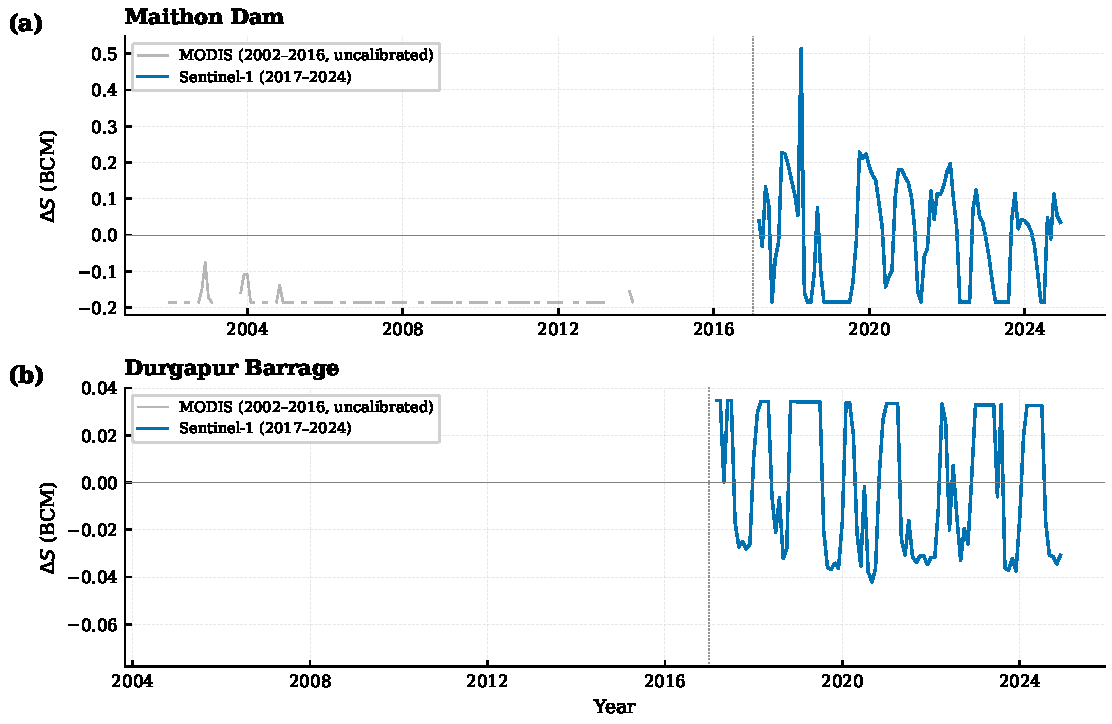
\includegraphics[width=0.9\linewidth]{Fig3_storage_timeseries}
  \caption{Reconstructed storage anomaly timeseries ($\dSobs$, BCM) for
  Maithon Dam (blue) and Durgapur Barrage (orange), 2017--2024. The distinct
  Rabi drawdown signature at Durgapur (October--March trough) and the 2018
  anomalous high-fill event at Maithon (peak $+0.51$ BCM) are visible.}
  \label{fig:thesis_storage_ts}
\end{figure}

\begin{figure}[htbp]
  \centering
  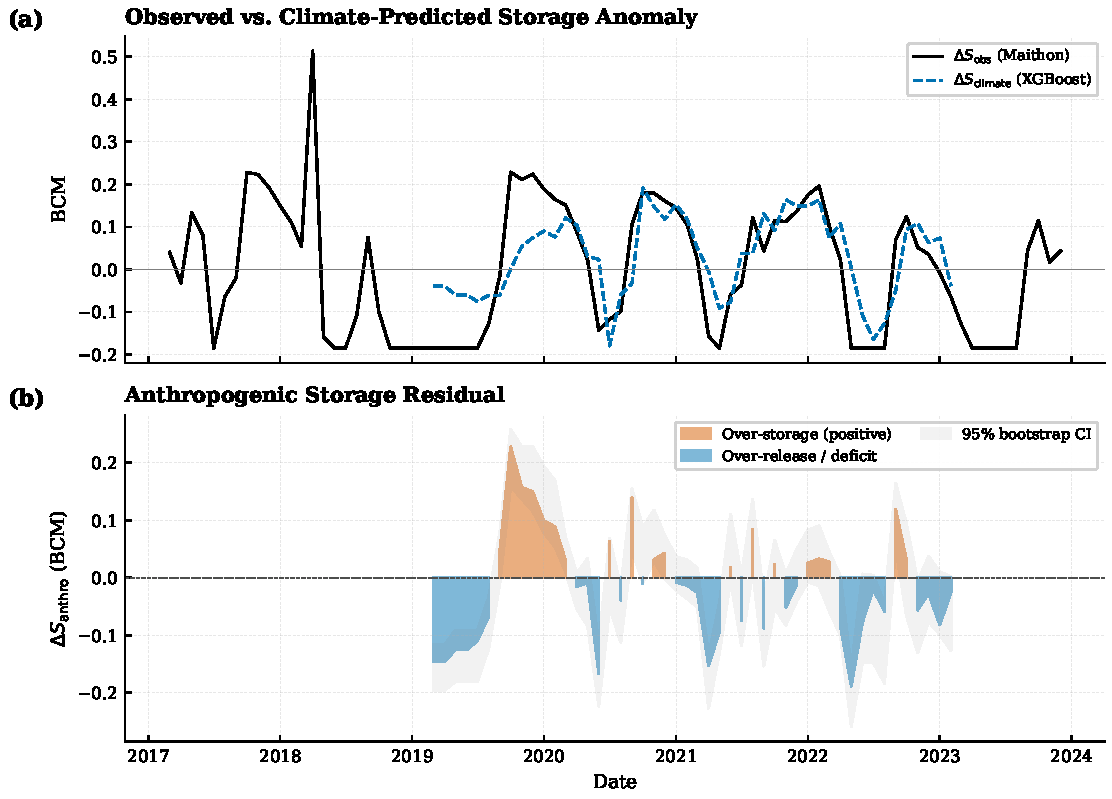
\includegraphics[width=0.9\linewidth]{Fig9_anthro_timeseries}
  \caption{Anthropogenic storage anomaly $\dSanthro$ for Maithon Dam. Red
  fill: DRAWDOWN state ($\dSanthro < 0$); blue fill: FILL state. HMM state
  assignments on lower axis (orange = DRAWDOWN, 25\% of months; grey =
  NORMAL, 75\%). Grey shading: seed-sensitivity envelope $\pm 0.051$ BCM.}
  \label{fig:thesis_anthro}
\end{figure}

\begin{figure}[htbp]
  \centering
  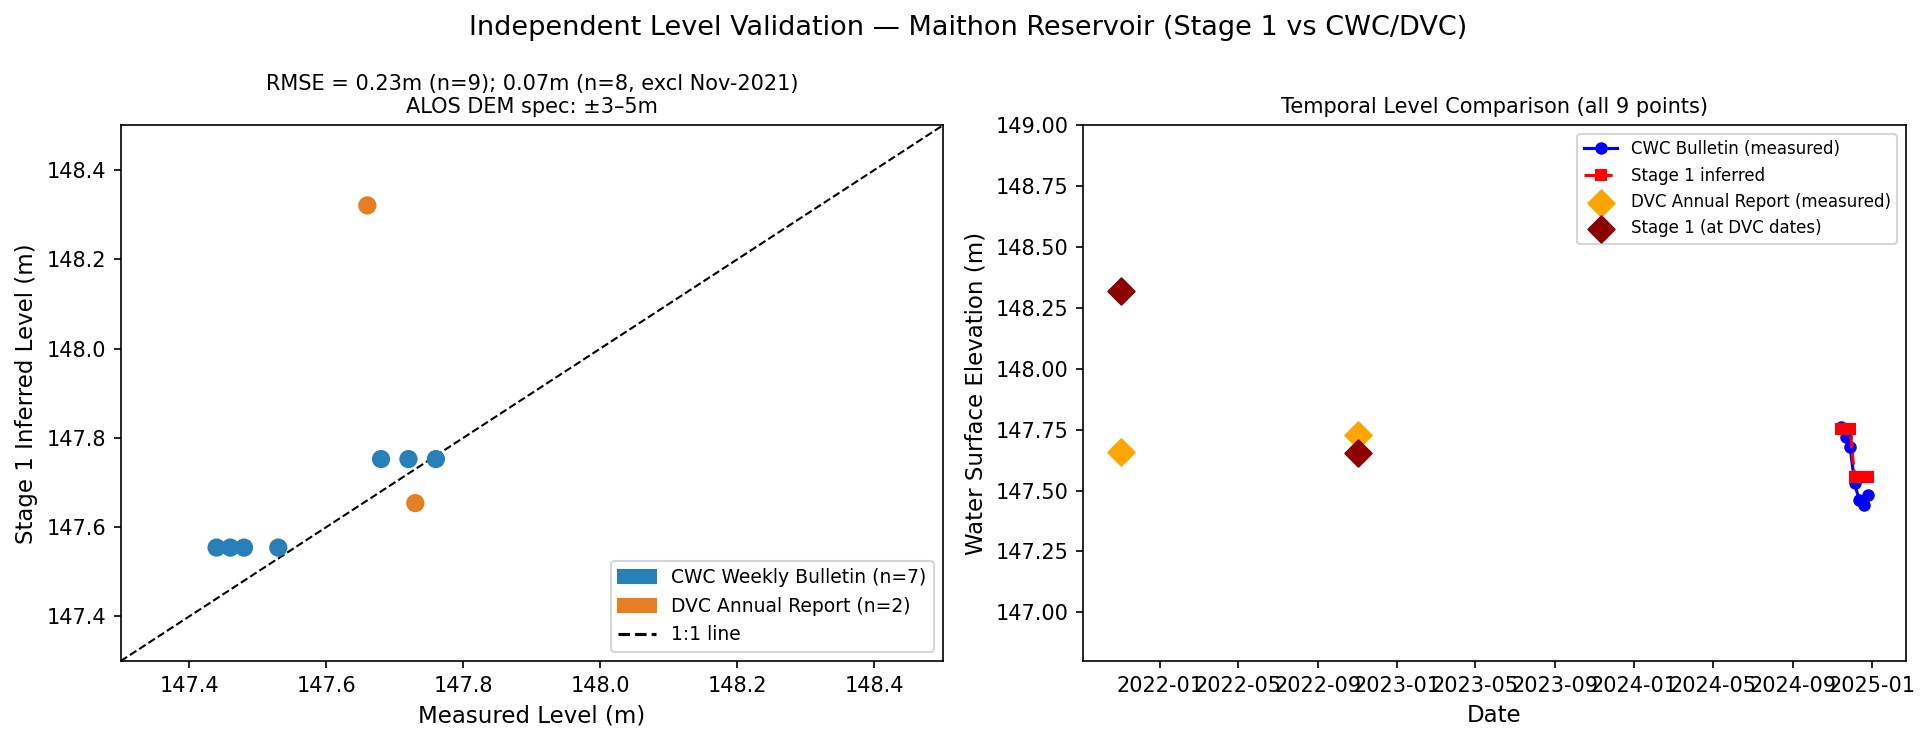
\includegraphics[width=0.9\linewidth]{FigS2_cwc_validation}
  \caption{CWC validation: measured vs Sentinel-1 inferred water surface
  elevation for Maithon ($n = 9$ independent points). RMSE = 0.07 m
  excluding the November 2021 temporal mismatch outlier.}
  \label{fig:thesis_cwc_validation}
\end{figure}

\begin{figure}[htbp]
  \centering
  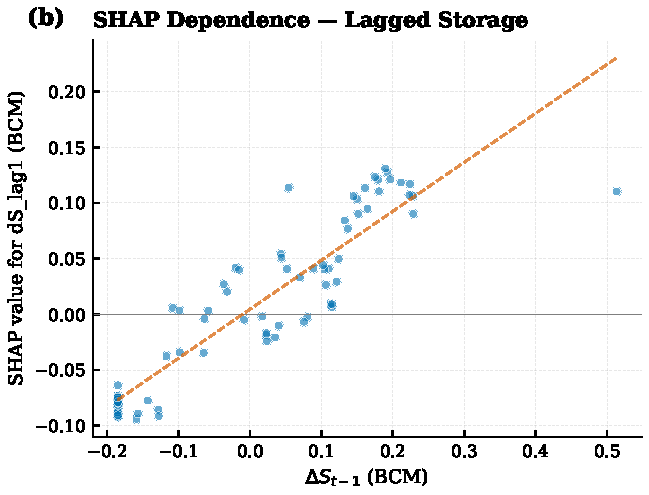
\includegraphics[width=0.9\linewidth]{Fig4b_SHAP_dependence_top}
  \caption{SHAP dependence plot for $\dS_{\text{lag1}}$, the dominant
  feature. The positive SHAP--feature correlation confirms that high
  prior-month storage predicts higher current storage, consistent with
  reservoir operational persistence.}
  \label{fig:thesis_shap_dep}
\end{figure}

\end{appendices}

\end{document}
